\section{Phân tích và Thiết kế Hệ thống}
\subsection{Kiến trúc Hệ thống}

Để trực quan hóa các luồng dữ liệu và sự phân tách vai trò giữa các thành phần công nghệ trong Hệ thống Quản lý Thư viện Trực tuyến, cấu trúc tổng thể được mô hình hóa qua sơ đồ kiến trúc dưới đây:

\begin{figure}[H]
	\centering
	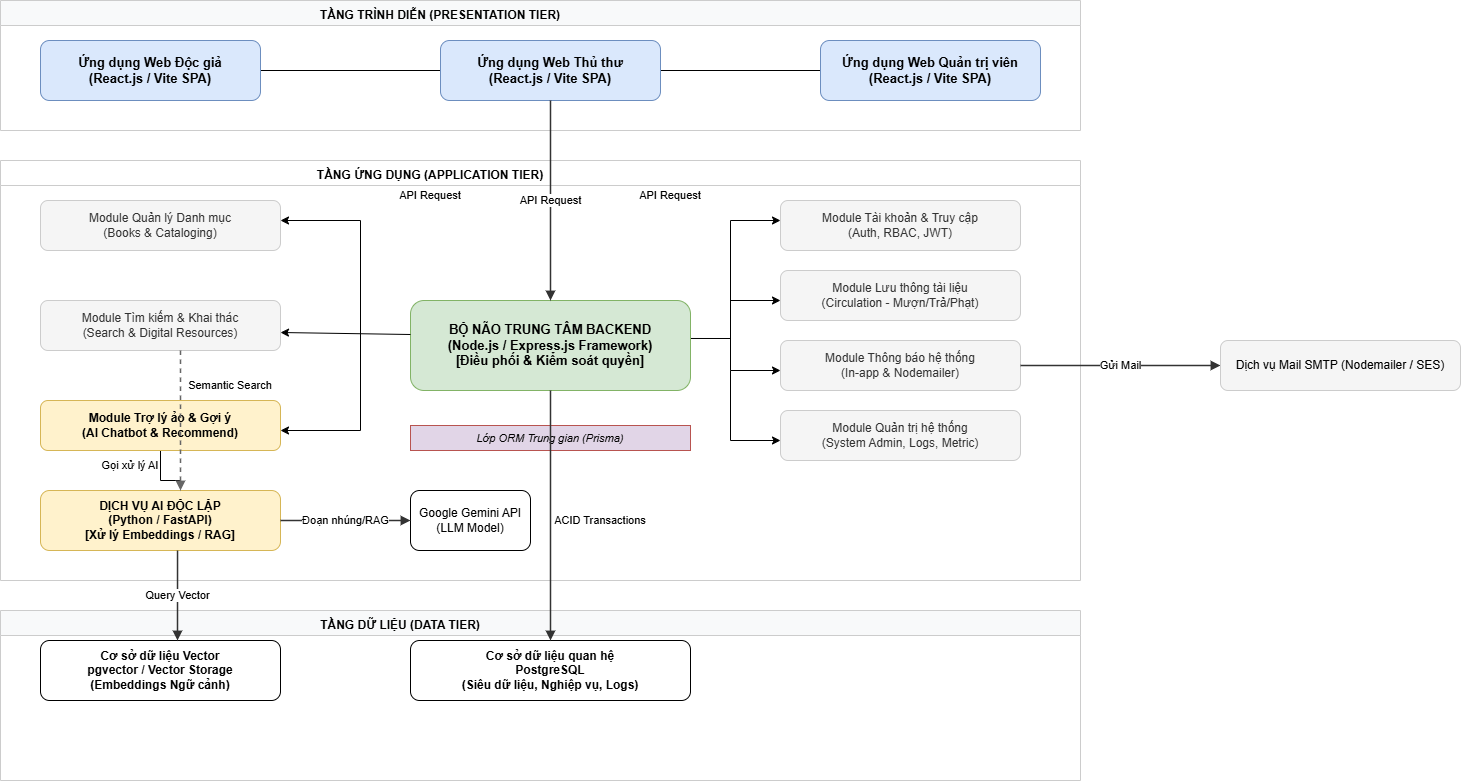
\includegraphics[width=0.6\linewidth]{Images/kientruchethong.png}
	\vspace{10pt}
	\caption{Sơ đồ Kiến trúc Tổng thể của Hệ thống Quản lý Thư viện Trực tuyến}
	\label{fig:system_architecture}
\end{figure}

Tổng thể, kiến trúc của Hệ thống Quản lý Thư viện Trực tuyến được xây dựng dựa trên Mô hình 3 Tầng tiêu chuẩn (Three-Tier Architecture), kết hợp linh hoạt với mô hình Kiến trúc Hướng Dịch vụ (SOA) để tối ưu hóa các tác vụ Trí tuệ Nhân tạo độc lập. Ba tầng nền tảng của dự án bao gồm: Tầng Giao diện (Presentation Tier), Tầng Ứng dụng (Application Tier) và Tầng Dữ liệu (Data Tier).

Việc áp dụng mô hình này đảm bảo sự phân tách rõ ràng trách nhiệm giữa tương tác giao diện người dùng, logic nghiệp vụ thư viện và các hệ quản trị cơ sở dữ liệu. Nhờ tính độc lập cao giữa các tầng, nhóm phát triển có thể dễ dàng bảo trì hoặc nâng cấp độc lập từng thành phần (như tối ưu hóa thuật toán AI hoặc cập nhật giao diện web) mà không làm gián đoạn các quy trình vận hành cốt lõi bên dưới.

\subsubsection{Tầng Giao diện (Presentation Tier)}
Đóng vai trò là điểm tiếp xúc trực tiếp cho người dùng cuối, tầng này được triển khai dưới dạng một Ứng dụng Trang Đơn (SPA) mạnh mẽ sử dụng thư viện React.js và công cụ đóng gói Vite. Giao diện được tùy chỉnh với cơ chế Kiểm soát Truy cập Dựa trên Vai trò (RBAC) nghiêm ngặt trên ba vai trò người dùng riêng biệt: Độc giả (Reader), Thủ thư (Librarian) và Quản trị viên (Admin).

Tất cả các tương tác của người dùng—bao gồm tìm kiếm tài liệu, gửi yêu cầu mượn trả, trò chuyện với trợ lý AI hoặc thực hiện các thao tác quản trị của thủ thư—đều được bắt giữ, xử lý bất đồng bộ và chuyển đổi thành các yêu cầu RESTful API tiêu chuẩn trước khi truyền đến tầng xử lý trung tâm.

\subsubsection{Tầng Ứng dụng (Application Tier)}
Hoạt động như trung tâm điều phối cốt lõi, Tầng Ứng dụng tiếp nhận, xử lý và thực thi các logic nghiệp vụ phức tạp cần thiết cho một hệ thống thư viện thông minh. Tầng này vận hành chủ yếu trong môi trường Node.js kết hợp với khung ứng dụng Express.js, đồng thời tích hợp một dịch vụ Python độc lập (FastAPI) chuyên trách các tác vụ AI hiệu năng cao. Để đảm bảo tính mô-đun và khả năng mở rộng, backend được chia thành 7 mô-đun chức năng tương ứng với các miền nghiệp vụ của hệ thống:

\begin{itemize}
	\item \textbf{Mô-đun Quản lý Tài khoản và Truy cập:} Bảo vệ an ninh hệ thống thông qua Kiểm soát Truy cập Dựa trên Vai trò (RBAC) kết hợp với băm mật khẩu. Hệ thống sử dụng JSON Web Token (JWT) để quản lý an toàn phiên làm việc của người dùng. Ngoài ra, mô-đun này quản lý hồ sơ cá nhân người dùng, mã xác thực OTP và nhật ký kiểm toán hoạt động cho độc giả và nhân viên thư viện.

	\item \textbf{Mô-đun Quản lý Danh mục Sách:} Tổ chức cấu trúc thể loại phân cấp (\texttt{Category}) và lưu trữ dữ liệu tả sách (\texttt{Book}). Phân hệ này hỗ trợ thủ thư biên mục tự động bằng cách tích hợp các API bên thứ ba (Open Library, Google Books API) để tự động lấy thông tin sách qua mã ISBN.

	\item \textbf{Mô-đun Quản lý Lưu thông Tài liệu:} Xử lý toàn bộ vòng đời mượn và trả sách vật lý. Phân hệ theo dõi tình trạng khả dụng trên giá của từng bản sao (\texttt{PhysicalCopy}) qua mã vạch, tự động hóa hàng chờ đặt chỗ (\texttt{Reservation}), tính toán điều kiện gia hạn trực tuyến, áp dụng các quy tắc phạt (\texttt{Fine}) cho các trường hợp quá hạn và điều phối chuyển sách liên chi nhánh.

	\item \textbf{Mô-đun Tìm kiếm và Khai thác Tài nguyên:} Cung cấp các bộ lọc tìm kiếm từ khóa và tìm kiếm ngữ nghĩa nâng cao để tối ưu hóa hiệu năng truy vấn trên toàn bộ danh mục sách.

	\item \textbf{Mô-đun Trợ lý Ảo và Gợi ý:} Vận hành như một microservice độc lập hiệu năng cao tận dụng các Mô hình Ngôn ngữ Lớn (LLM) thông qua Google Generative AI (Gemini API). Các khả năng bao gồm: Tìm kiếm Ngữ nghĩa theo ngôn ngữ tự nhiên, tóm tắt tài liệu tự động bằng AI, các thuật toán dự đoán sở thích để gợi ý cá nhân hóa và Chatbot Trợ lý ảo hỗ trợ 24/7.

	\item \textbf{Mô-đun Thông báo:} Tự động hóa truyền thông người dùng theo thời gian thực. Hệ thống lắng nghe các sự kiện hệ thống (nhắc nhở hạn trả, tính phí phạt, thông báo sách đặt chỗ đã về) để phát thông báo đa kênh qua cảnh báo trong ứng dụng và email tự động sử dụng Nodemailer.

	\item \textbf{Mô-đun Quản trị Hệ thống:} Cung cấp các công cụ quản trị cho việc quản lý hệ thống, bao gồm các cặp khóa-giá trị cấu hình hệ thống động (\texttt{system\_configs}), quản lý mạng lưới chi nhánh, bảng điều khiển chỉ số theo thời gian thực (\texttt{Dashboard Metrics}), sao lưu cơ sở dữ liệu tự động và khôi phục sự cố.
\end{itemize}

Để tối đa hóa tốc độ phát triển và tính an toàn kiểu dữ liệu, Tầng Ứng dụng sử dụng \textbf{Prisma ORM} làm tầng truy cập dữ liệu. Tận dụng khả năng kiểm tra kiểu tĩnh nghiêm ngặt của TypeScript, Prisma giúp phát hiện các lỗi cú pháp truy vấn ngay trong quá trình biên dịch. Prisma Migrate quản lý các phiên bản lược đồ cơ sở dữ liệu, đảm bảo sự đồng bộ lược đồ tự động giữa môi trường phát triển và sản xuất.

\subsubsection{Tầng Dữ liệu (Data Tier)}
Tầng lưu trữ dữ liệu cung cấp khả năng lưu trữ bền vững, an toàn và tuân thủ nguyên tắc ACID cho tất cả các bản ghi của hệ thống. Tầng này bao gồm hai kho cơ sở dữ liệu chuyên biệt:

\begin{itemize}
	\item \textbf{Cơ sở Dữ liệu Quan hệ (PostgreSQL):} Đối với các thao tác thư viện đòi hỏi độ chính xác giao dịch tài chính nghiêm ngặt và tính nhất quán đồng thời (ví dụ: giảm số lượng kho vật lý đồng thời tạo phiếu mượn), \textbf{PostgreSQL} được lựa chọn nhờ tuân thủ ACID mạnh mẽ. Cấu trúc chỉ mục hiệu năng cao đảm bảo độ trễ thấp dưới tải truy vấn lớn. Ngoài ra, tất cả các hành động thay đổi trạng thái nhạy cảm đều ghi tự động các bản ghi vào nhật ký kiểm toán (\texttt{AuditLog}).

	\item \textbf{Cơ sở Dữ liệu Vector (pgvector):} Để phục vụ Mô hình Tạo Xuất Kiến thức Kết hợp Truy vấn (RAG) và tìm kiếm ngữ nghĩa trong các mô-đun AI, tầng dữ liệu tích hợp các cơ chế lưu trữ vector. Các tóm tắt văn bản, dữ liệu tả sách và các đoạn tài liệu số được chuyển đổi thành các vector nhúng nhiều chiều được lưu trữ và truy vấn bằng độ tương đồng Cosine trực tiếp trong `pgvector`.
\end{itemize}

\subsection{Thiết kế Cơ sở Dữ liệu}
\subsubsection{Mô tả Thực thể}

\begin{table}[H]
	\centering
	\begin{tabular}{|p{4cm}|p{4cm}|p{7cm}|}
		\hline
		\textbf{Nhóm Thực thể} & \textbf{Tên Thực thể}   & \textbf{Mô tả}                                                                   \\ \hline

		\multirow{5}{*}{Người dùng \& Kiểm soát Truy cập}
		                         & users                  & Lưu trữ hồ sơ tài khoản người dùng bao gồm độc giả, thủ thư và quản trị viên. \\ \cline{2-3}
		                         & roles                  & Quản lý vai trò hệ thống và phân quyền (Admin, Librarian, Reader).         \\ \cline{2-3}
		                         & otp\_tokens            & Lưu trữ mã OTP cho xác thực đăng nhập, đặt lại mật khẩu và MFA.                  \\ \cline{2-3}
		                         & notification\_settings & Lưu trữ tùy chọn thông báo của người dùng qua Email, SMS và In-app.           \\ \cline{2-3}
		                         & notifications          & Quản lý thông báo hệ thống gửi đến người dùng (cảnh báo hạn trả, thông báo đặt chỗ).      \\ \hline

		\multirow{5}{*}{Tài nguyên Thư viện}
		                         & books                  & Lưu trữ các bản ghi dữ liệu tả cho sách, tạp chí và tài liệu học thuật số.           \\ \cline{2-3}
		                         & categories             & Quản lý phân loại thể loại theo phân cấp cho các chủ đề và ngành học.            \\ \cline{2-3}
		                         & physical\_copies       & Theo dõi các bản sao vật lý, trạng thái lưu thông và vị trí kệ sách.             \\ \hline

		\multirow{5}{*}{Lưu thông Thư viện}
		                         & borrow\_records        & Theo dõi vòng đời mượn và trả tài liệu vật lý.                          \\ \cline{2-3}
		                         & reservations           & Quản lý hàng chờ đặt giữ chỗ tài liệu khi hết bản sao khả dụng.                     \\ \cline{2-3}
		                         & fines                  & Quản lý phí phạt quá hạn và các khoản phí vi phạm.                                     \\ \cline{2-3}
		                         & branches               & Lưu trữ thông tin chi nhánh thư viện và dữ liệu tả vị trí cơ sở.                           \\ \cline{2-3}
		                         & branch\_transfers      & Quản lý việc chuyển bản sao vật lý giữa các chi nhánh thư viện.                              \\ \hline

		\multirow{2}{*}{Tương tác \& Đánh giá}
		                         & reviews                & Lưu trữ đánh giá 5 sao, nhận xét và phản hồi của người dùng về tài liệu.                       \\ \cline{2-3}
		                         & chat\_history          & Lưu trữ lịch sử hội thoại giữa người dùng và Chatbot trợ lý AI.            \\ \hline

		\multirow{2}{*}{Hệ thống \& Quản trị}
		                         & audit\_logs            & Ghi lại các sự kiện kiểm toán quản trị và an ninh cho tuân thủ hệ thống.                \\ \cline{2-3}
		                         & system\_configs        & Lưu trữ các tham số cấu hình động toàn cục cho vận hành hệ thống.                   \\ \hline
	\end{tabular}
	\caption{Các Thực thể Hệ thống và Định nghĩa Cơ sở Dữ liệu}
	\label{tab:entity-description}
\end{table}

\subsubsection{Sơ đồ Thực thể Phân cấp Nâng cao (EERD)}

\begin{figure}[H]
	\centering
	\includegraphics[width=\linewidth]{Images/ERD.png}
	\vspace{10pt}
	\caption{Sơ đồ EERD của Hệ thống Quản lý Thư viện Trực tuyến}
	\label{fig:erd_account}
\end{figure}

Dựa trên Sơ đồ Thực thể Phân cấp Nâng cao (EERD), các quy trình vận hành hệ thống được chia thành ba vai trò người dùng chính:

\paragraph{Vai trò Độc giả (Reader)}
Người dùng cuối tương tác với nền tảng để tìm kiếm, mượn và đọc các tài liệu in và tài liệu số:
\begin{itemize}
	\item \textbf{Quản lý Tài khoản \& An ninh:} Thực thi xác thực đa yếu tố qua mã OTP (\texttt{otp\_tokens}); cấu hình các kênh thông báo (Email, SMS, In-app) trong \texttt{notification\_settings}.
	\item \textbf{Mượn Vật lý \& Tra cứu Danh mục:} Tìm kiếm và duyệt danh mục thể loại (\texttt{categories}). Mượn tài liệu vật lý với bản ghi mượn được theo dõi trong \texttt{borrow\_records}.
	\item \textbf{Mượn \& Trả Vật lý:} Gửi yêu cầu mượn và theo dõi vòng đời mượn trong \texttt{borrow\_records} gắn với từng bản sao cụ thể (\texttt{physical\_copies}).
	\item \textbf{Quản lý Hàng chờ Đặt chỗ:} Khi sách hết bản sao khả dụng, thực hiện đặt giữ chỗ (\texttt{reservations}) với vị trí hàng chờ tự động qua \texttt{queuePosition}.
	\item \textbf{Phản hồi \& Đánh giá:} Gửi đánh giá sao và nhận xét (\texttt{reviews}); trò chuyện với Trợ lý Ảo AI (\texttt{chat\_history}); xem và thanh toán tiền phạt (\texttt{fines}).
\end{itemize}

\paragraph{Vai trò Thủ thư (Librarian)}
Nhân viên vận hành quản lý kho sách vật lý, các bản ghi danh mục và quầy lưu thông:
\begin{itemize}
	\item \textbf{Quản lý Kho Sách Vật lý:} Quản lý các bản ghi danh mục (\texttt{books}), tình trạng khả dụng của bản sao (\texttt{status}), tình trạng vật lý (\texttt{condition}) và vị trí kệ (\texttt{location}) trong \texttt{physical\_copies}.
	\item \textbf{Xử lý tại Quầy Lưu thông:} Quét mã vạch (\texttt{barcode}) và thẻ độc giả (\texttt{readerCode}), cập nhật \texttt{borrow\_records}.
	\item \textbf{Điều phối Hàng chờ Đặt chỗ:} Giám sát hàng chờ đặt chỗ (\texttt{reservations}), cập nhật trạng thái bản sao khi được trả và thông báo cho người dùng tiếp theo.
	\item \textbf{Vận chuyển Liên Chi nhánh:} Duyệt và theo dõi phiếu chuyển sách giữa các chi nhánh thư viện qua \texttt{branch\_transfers}.
	\item \textbf{Tính và Miễn Phí Phạt:} Xem xét các khoản phạt quá hạn trong \texttt{fines}, có thẩm quyền miễn giảm phạt (\texttt{waivedById}, \texttt{waivedReason}).
\end{itemize}

\paragraph{Vai trò Quản trị viên (Admin)}
Quản trị viên hệ thống nắm giữ các quyền cấu hình toàn cục, an ninh người dùng và kiểm toán:
\begin{itemize}
	\item \textbf{Quản lý Người dùng \& RBAC:} Kích hoạt, khóa hoặc đình chỉ tài khoản (\texttt{users}), quản lý giới hạn đăng nhập thất bại (\texttt{failedLoginCount}) và phân quyền vai trò (\texttt{roles}).
	\item \textbf{Quản trị Hạ tầng:} Quản lý cấu hình mạng lưới chi nhánh (\texttt{branches}) và gán người quản lý chi nhánh (\texttt{managerId}).
	\item \textbf{Tham số Toàn cục:} Cấu hình các chính sách vận hành hệ thống qua \texttt{system\_configs} (mức phạt hằng ngày, hạn mức mượn, kích thước tệp tải lên tối đa).
	\item \textbf{Kiểm toán Hệ thống:} Giám sát nhật ký kiểm toán (\texttt{audit\_logs}) để đảm bảo an toàn dữ liệu và tuân thủ quy định.
\end{itemize}

\subsubsection{Lược đồ Cơ sở Dữ liệu}
\begin{figure}[H]
	\centering
	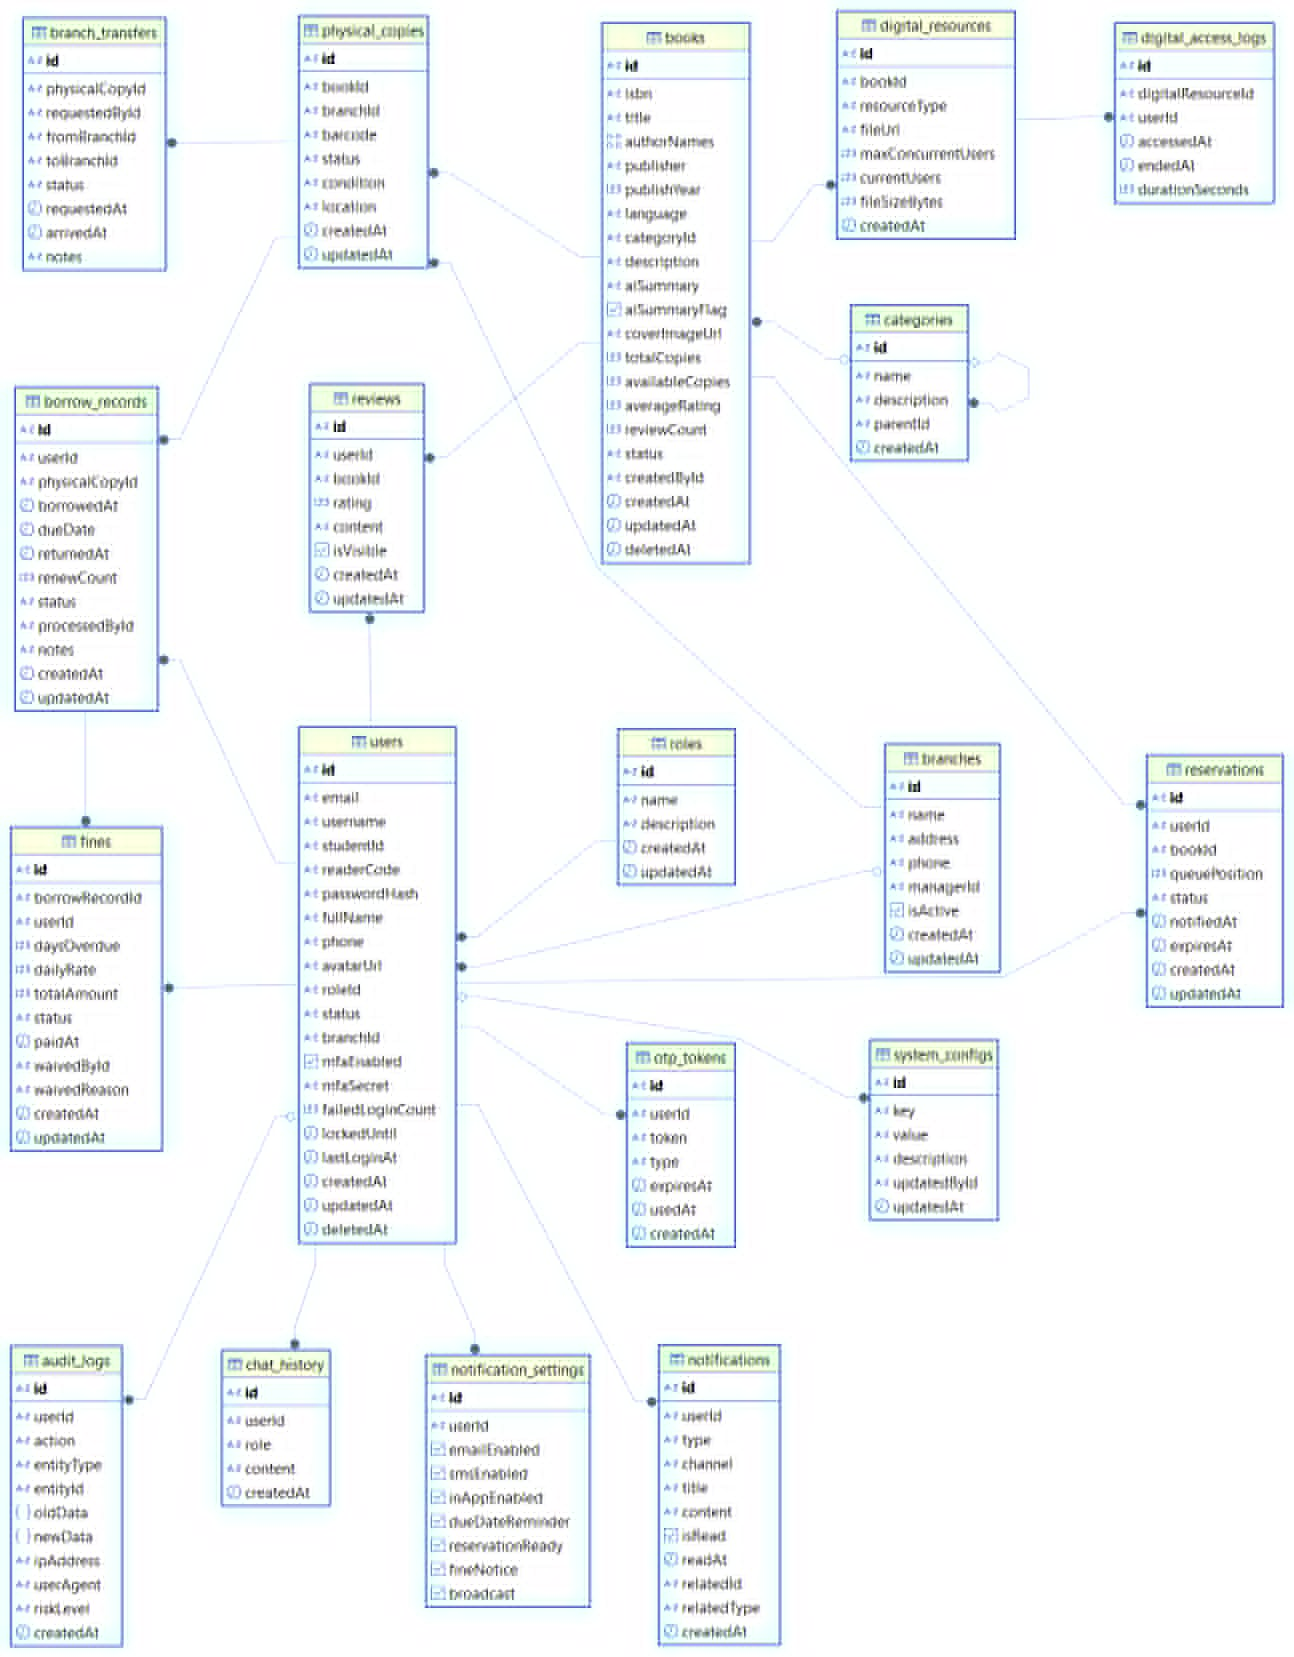
\includegraphics[width=0.6\linewidth]{Images/db.jpg}
	\vspace{10pt}
	\caption{Lược đồ Cơ sở Dữ liệu Quan hệ của Hệ thống Quản lý Thư viện Trực tuyến}
	\label{fig:database_account}
\end{figure}
Lược đồ trên đại diện cho cấu trúc quan hệ được triển khai trên PostgreSQL.

Tài khoản người dùng được tập trung trong bảng \texttt{users}, liên kết với \texttt{roles} qua khóa ngoại \texttt{roleId} để kiểm tra quyền RBAC. Các cờ an ninh như \texttt{status}, \texttt{failedLoginCount}, và \texttt{lockedUntil} thực thi các ràng buộc an ninh đăng nhập.

Các bảng còn lại ánh xạ trực tiếp tới các định nghĩa thực thể và quan hệ EERD đã mô tả ở trên.

\subsection{Sơ đồ Lớp (Class Diagram)}

\subsubsection{Quản lý Tài khoản và Truy cập}

\begin{figure}[H]
	\centering
	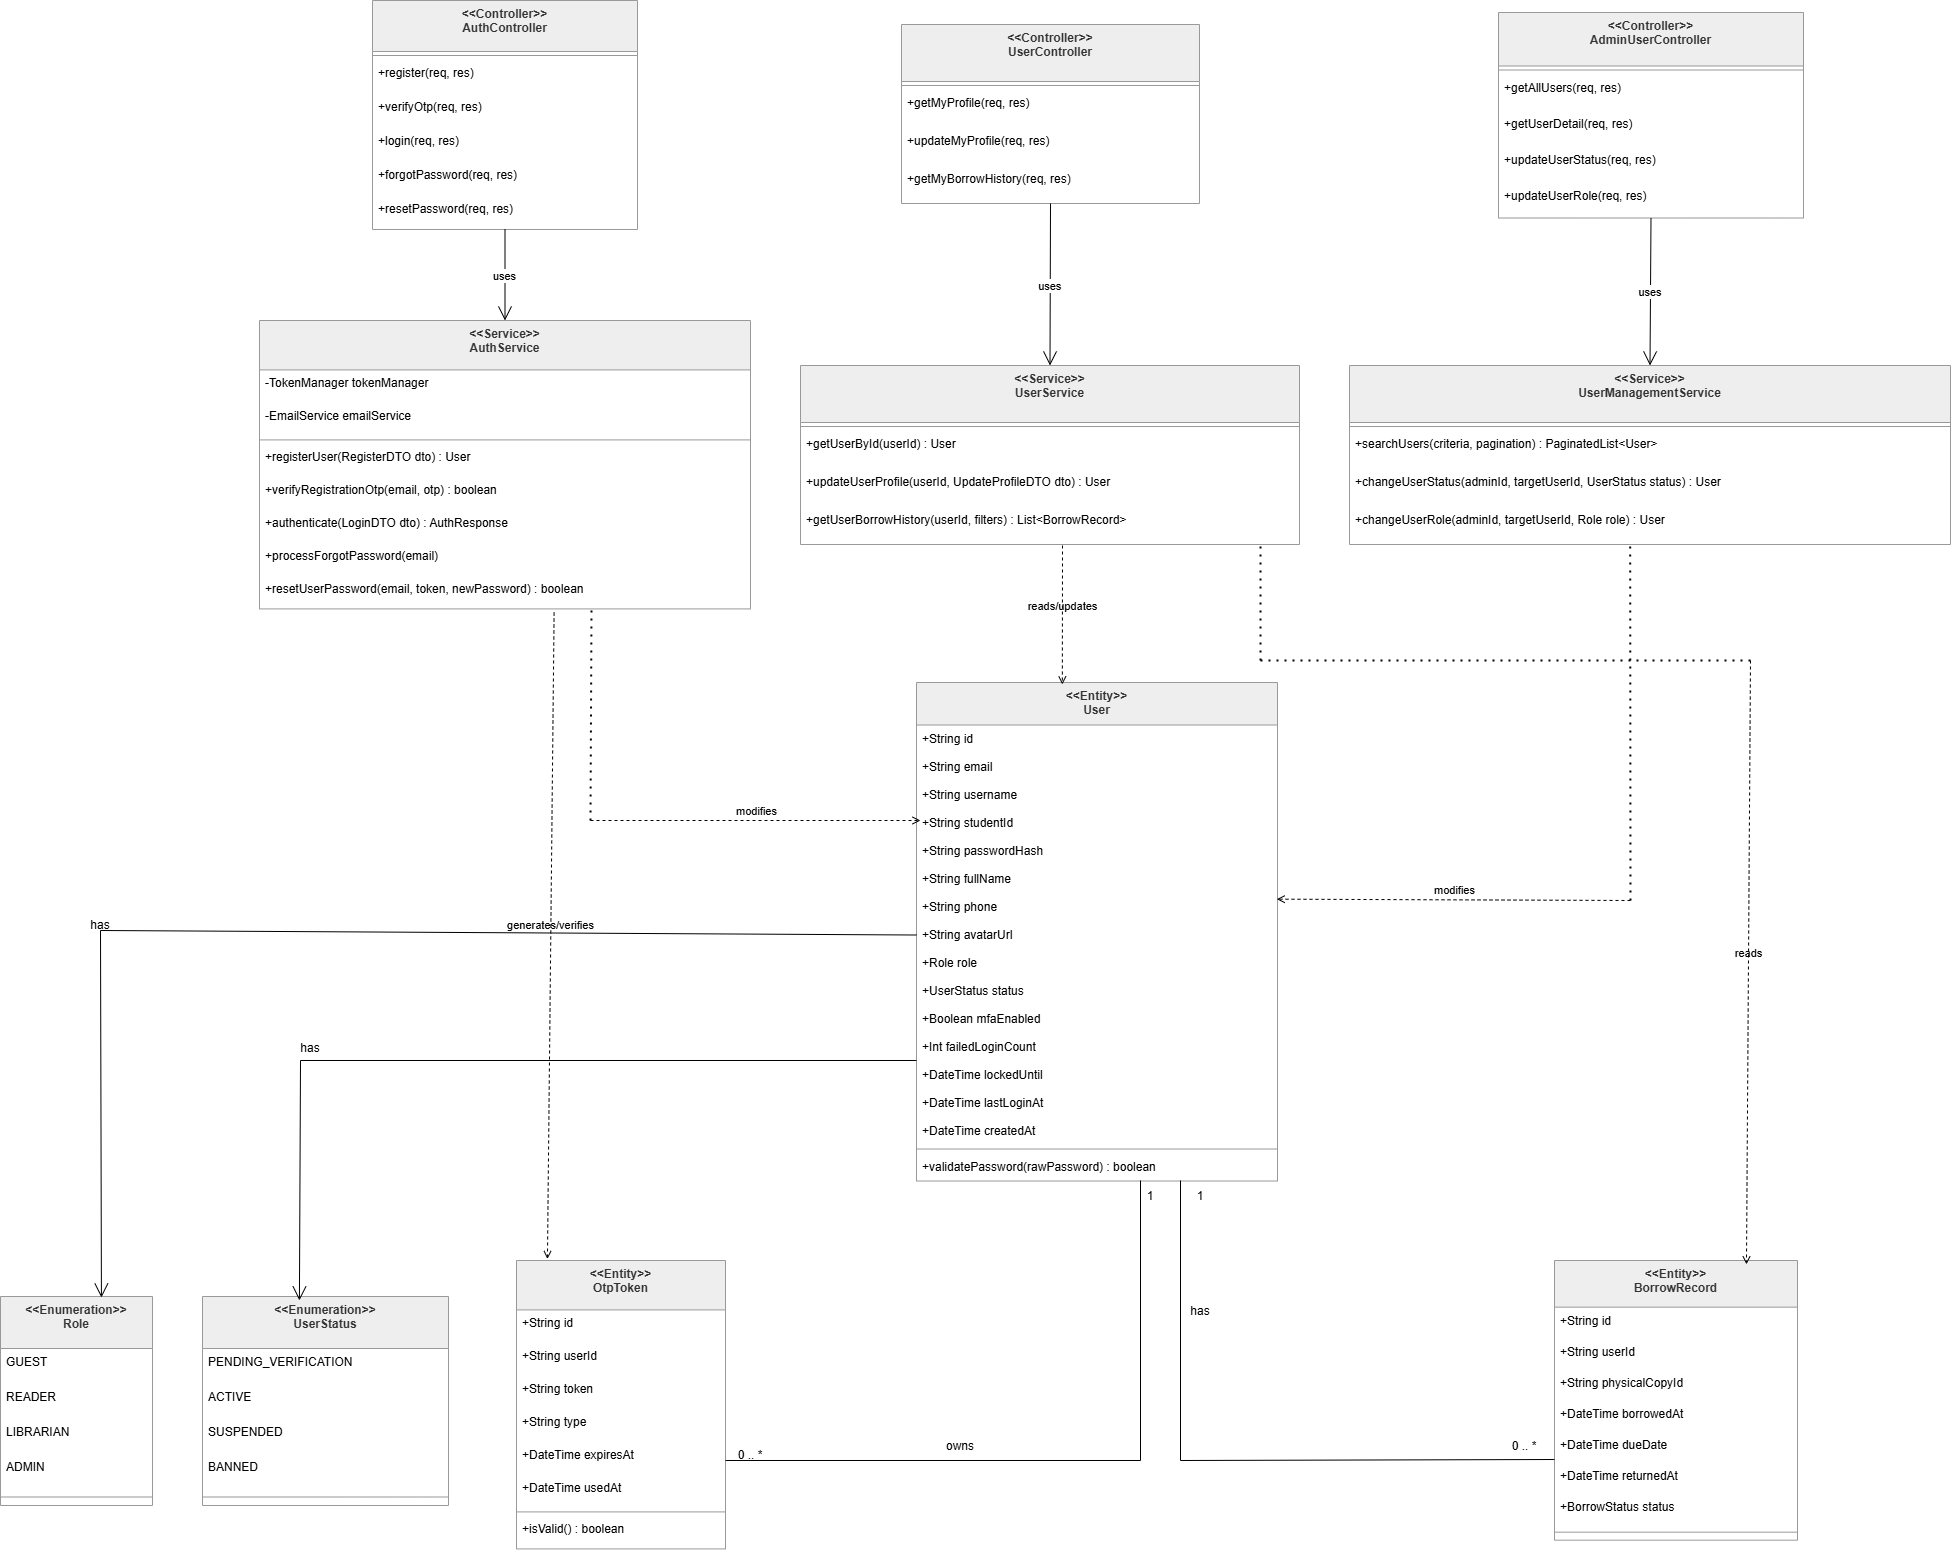
\includegraphics[width=0.6\linewidth]{Images/quanlytruycapvataikhoan.png}
	\vspace{10pt}
	\caption{Sơ đồ Lớp cho Quản lý Tài khoản và Truy cập}
	\label{fig:class_account}
\end{figure}

Sơ đồ lớp \textbf{Quản lý Tài khoản và Truy cập} mô hình hóa cấu trúc đối tượng, thuộc tính và phương thức cho xác thực và quản lý hồ sơ.

Thực thể trung tâm là \texttt{User}, chứa các thuộc tính \texttt{id}, \texttt{email}, \texttt{username}, \texttt{fullName}, \texttt{phone}, \texttt{avatarUrl}, \texttt{studentId}, cùng các thuộc tính an ninh \texttt{passwordHash}, \texttt{mfaEnabled}, \texttt{failedLoginCount}, \texttt{lockedUntil}, \texttt{lastLoginAt} và \texttt{createdAt}. Phương thức cốt lõi \texttt{validatePassword(rawPassword)} thực hiện xác minh thông tin đăng nhập.

\texttt{User} liên kết với \texttt{Role} (GUEST, READER, LIBRARIAN, ADMIN) và \texttt{UserStatus} (PENDING\_VERIFICATION, ACTIVE, SUSPENDED, BANNED). \texttt{User} liên kết $1 - 0..*$ với \texttt{OtpToken} (phương thức \texttt{isValid()}) và $1 - 0..*$ với \texttt{BorrowRecord}.

Về mặt kiến trúc, \texttt{AuthController} phụ thuộc vào \texttt{AuthService} (\texttt{registerUser}, \texttt{verifyRegistrationOtp}, \texttt{authenticate}, \texttt{processForgotPassword}, \texttt{resetPasswordUser}). \texttt{UserController} phụ thuộc vào \texttt{UserService} (\texttt{getUserById}, \texttt{updateUserProfile}, \texttt{getUserBorrowHistory}). \texttt{AdminUserController} sử dụng \texttt{UserManagementService} (\texttt{searchUsers}, \texttt{getUserDetail}, \texttt{changeUserStatus}, \texttt{changeUserRole}).

\subsubsection{Quản lý Danh mục Sách}

\begin{figure}[H]
	\centering
	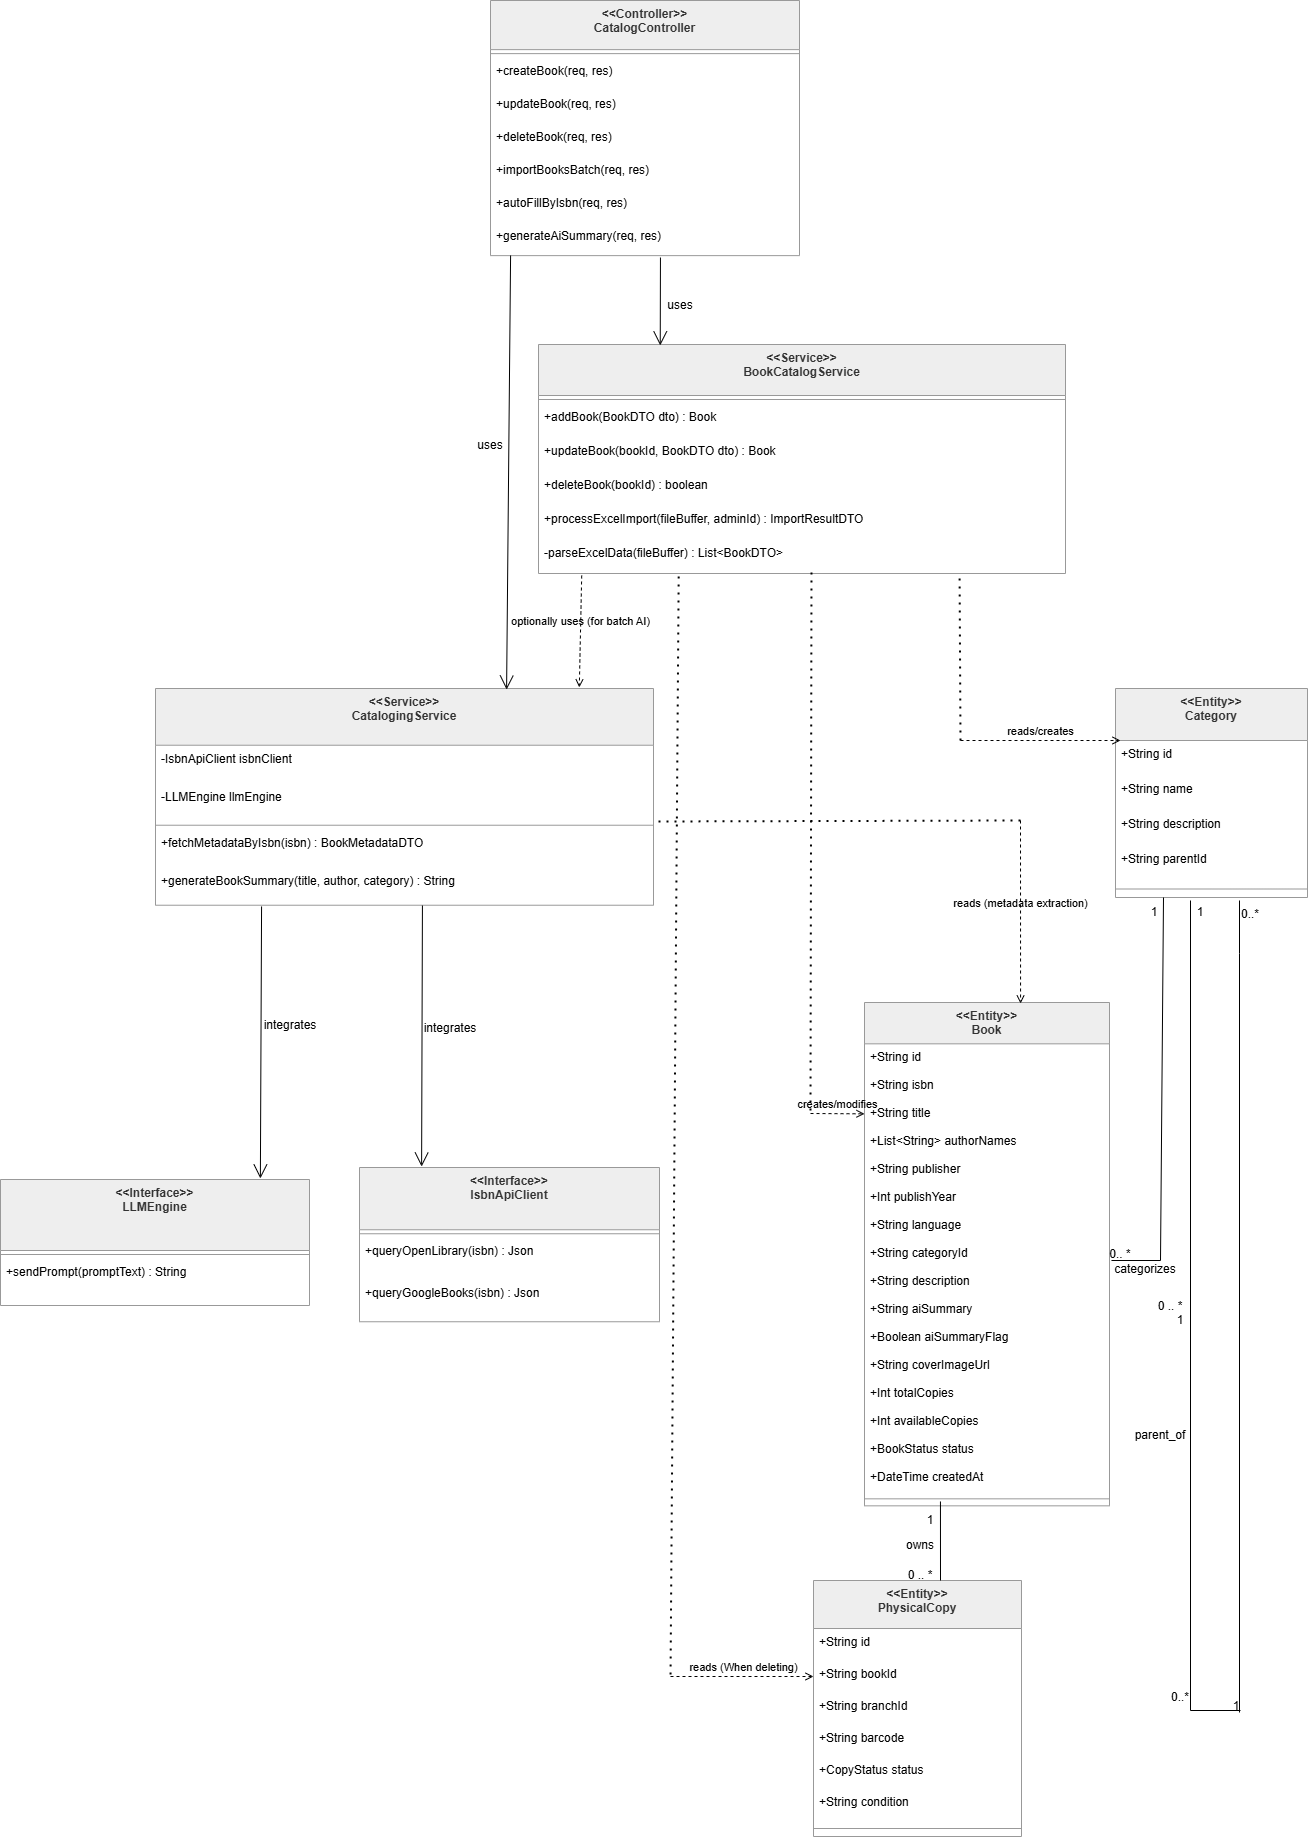
\includegraphics[width=0.6\linewidth]{Images/quanlydanhmuc.png}
	\vspace{10pt}
	\caption{Sơ đồ Lớp cho Quản lý Danh mục Sách}
	\label{fig:class_catalog}
\end{figure}

Các cấu trúc dữ liệu cốt lõi bao gồm \texttt{Category}, \texttt{Book} và \texttt{PhysicalCopy}. \texttt{Category} sở hữu phân cấp tự tham chiếu ($1 \to 0..\ast$) qua \texttt{parentId} và liên kết $1 \to 0..\ast$ với \texttt{Book}.

\texttt{Book} chứa dữ liệu tả danh mục (\texttt{isbn}, \texttt{title}, \texttt{authorNames}, \texttt{publisher}, \texttt{publishYear}, \texttt{language}, \texttt{totalCopies}, \texttt{availableCopies}, \texttt{aiSummary}) và liên kết $1 \to 0..\ast$ với \texttt{PhysicalCopy} (\texttt{barcode}, \texttt{CopyStatus status}, \texttt{condition}).

\texttt{CatalogController} ủy quyền cho \texttt{BookCatalogService} (\texttt{addBook}, \texttt{updateBook}, \texttt{deleteBook}, \texttt{autoFillByIsbn}, \texttt{generateAiSummary}, \texttt{processExcelImport}). \texttt{BookCatalogService} tương tác với \texttt{CatalogingService}, lớp bọc \texttt{IsbnApiClient} (\texttt{queryOpenLibrary}, \texttt{queryGoogleBooks}) và \texttt{LLMEngine} (\texttt{generateBookSummary}) cho biên mục tự động.

\subsubsection{Quản lý Lưu thông Tài liệu}

\begin{figure}[H]
	\centering
	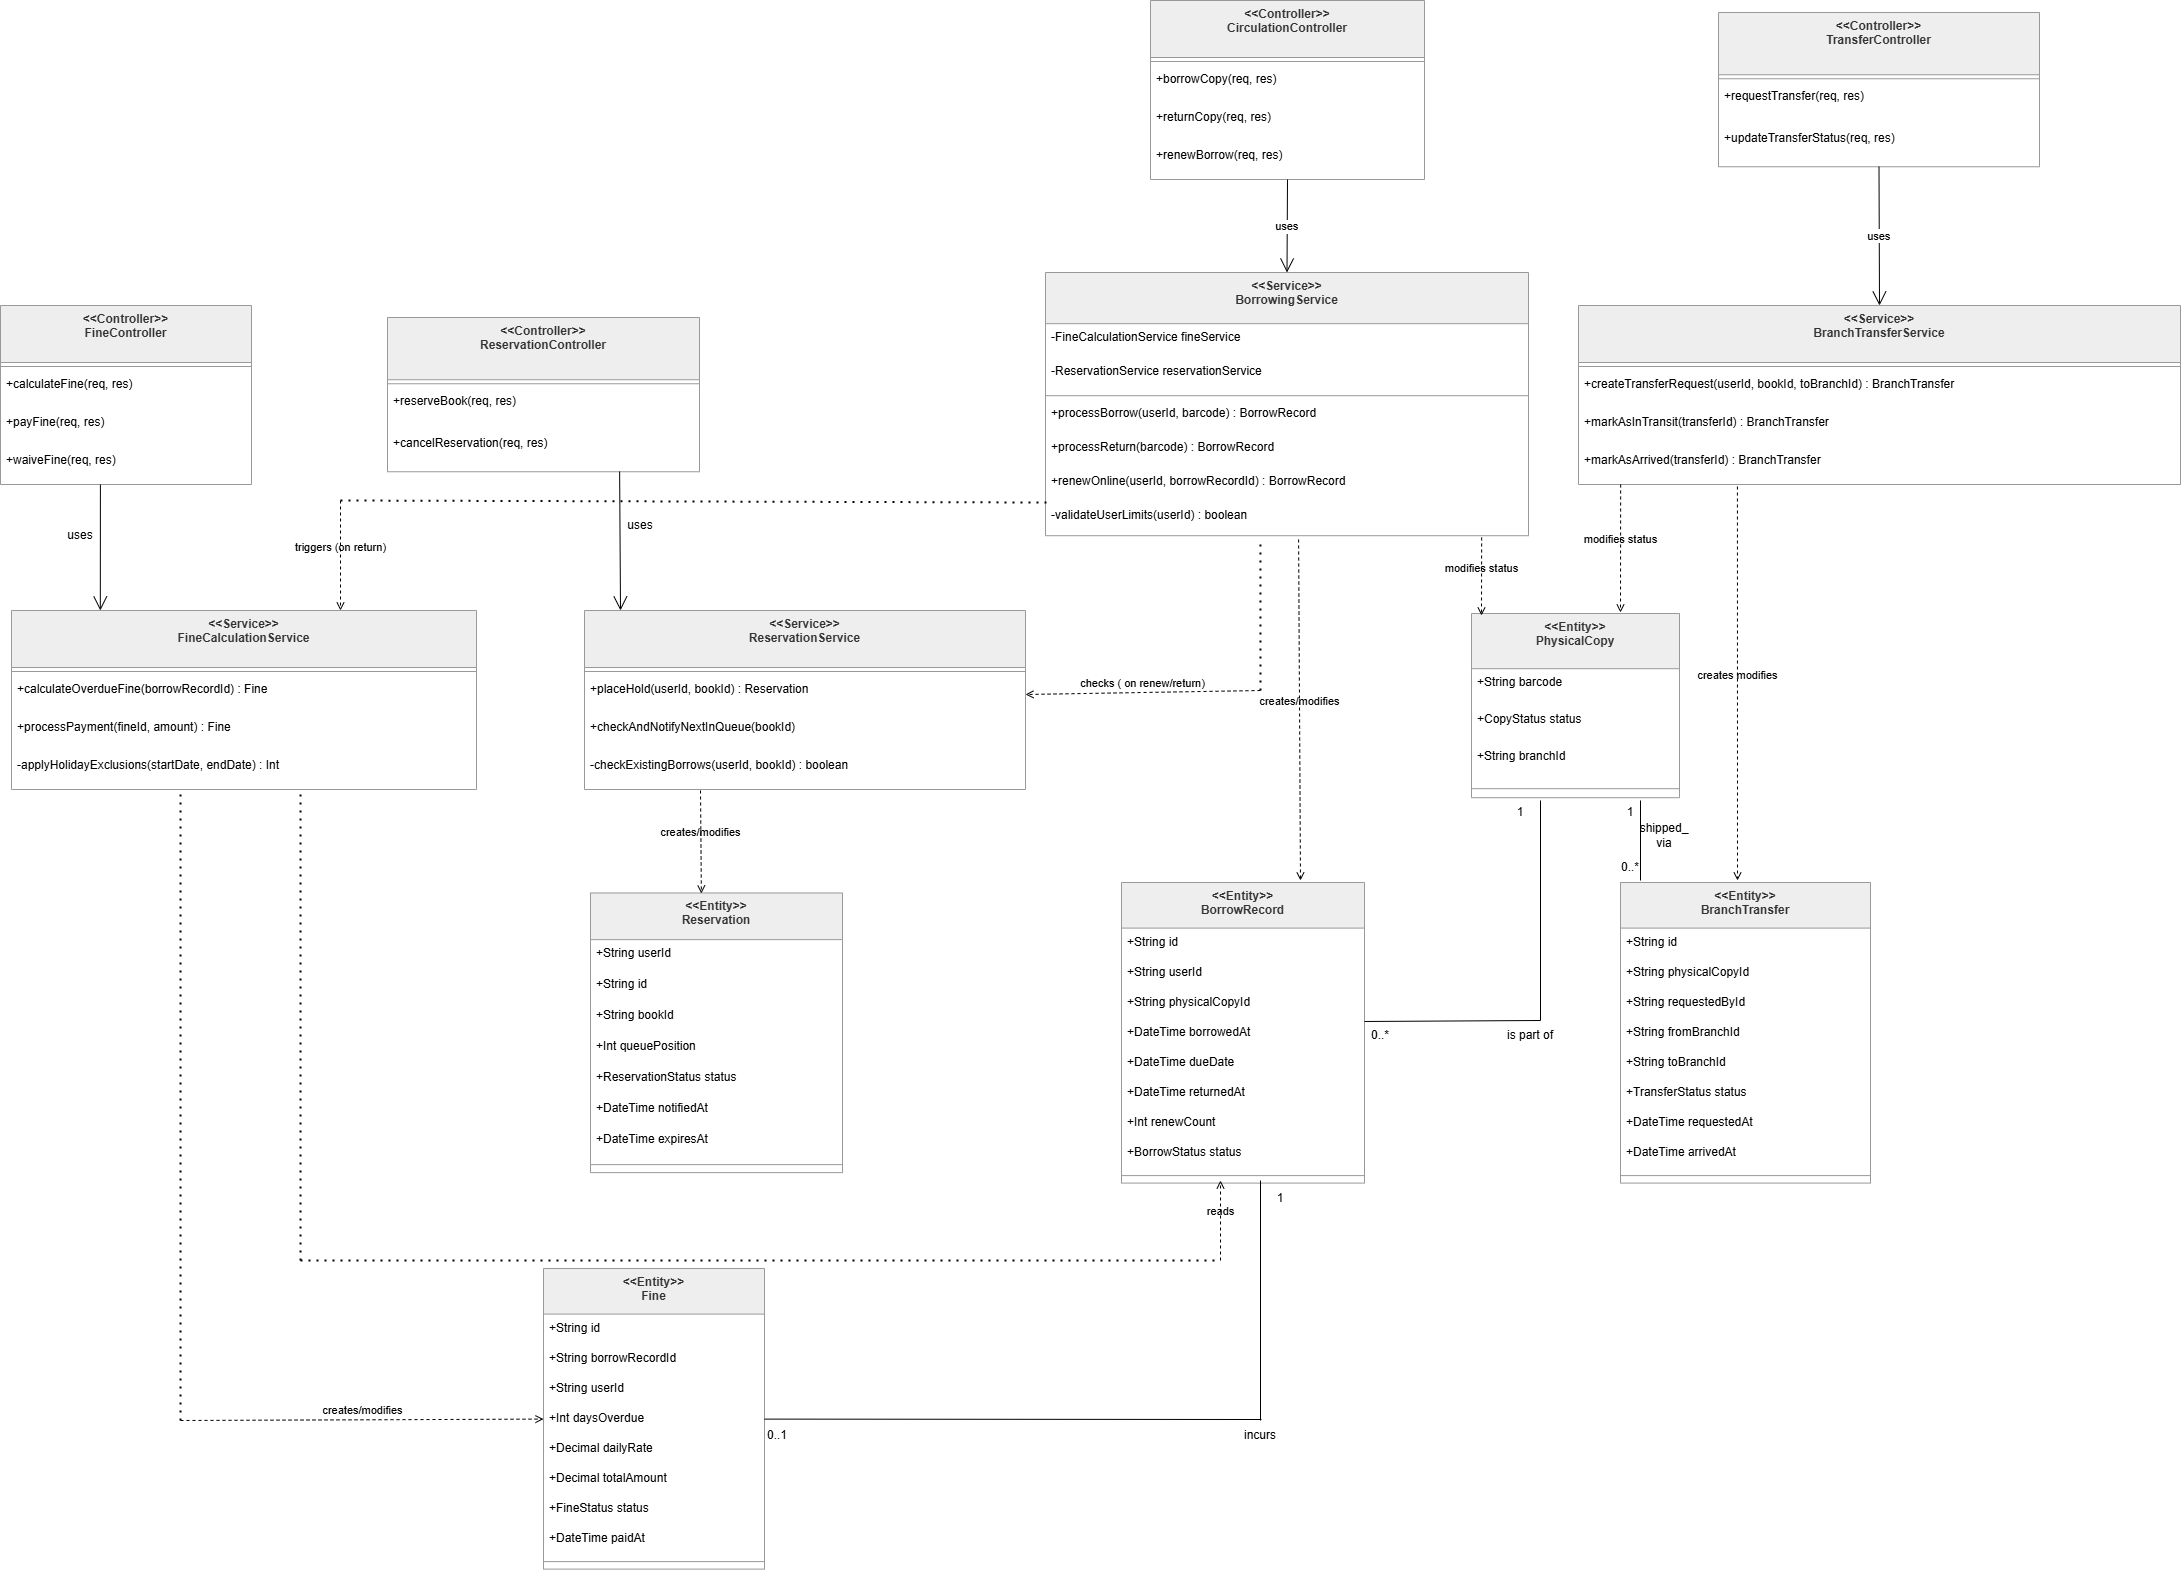
\includegraphics[width=0.6\linewidth]{Images/quanlyluuthong.png}
	\vspace{10pt}
	\caption{Sơ đồ Lớp cho Quản lý Lưu thông Tài liệu}
	\label{fig:class_circulation}
\end{figure}

Thực thể trung tâm \texttt{BorrowRecord} (\texttt{borrowedAt}, \texttt{dueDate}, \texttt{returnedAt}, \texttt{renewCount}, \texttt{BorrowStatus status}) liên kết với \texttt{PhysicalCopy} ($1 - 0..*$). \texttt{Reservation} (\texttt{queuePosition}, \texttt{ReservationStatus status}) và \texttt{Fine} ($1 - 0..1$ với \texttt{BorrowRecord}) xử lý hàng chờ đặt chỗ và tính phạt. \texttt{BranchTransfer} theo dõi việc chuyển sách giữa các chi nhánh.

\texttt{CirculationController} sử dụng \texttt{BorrowingService} (\texttt{processBorrow}, \texttt{processReturn}, \texttt{renewOnline}). \texttt{ReservationController} sử dụng \texttt{ReservationService} (\texttt{placeHold}, \texttt{cancelReservation}). \texttt{FineController} sử dụng \texttt{FineCalculationService} (\texttt{calculateOverdueFine}, \texttt{processPayment}). \texttt{TransferController} sử dụng \texttt{BranchTransferService} (\texttt{createTransferRequest}, \texttt{markInTransit}, \texttt{markAsArrived}).

\subsubsection{Tìm kiếm và Khai thác Tài nguyên}

\begin{figure}[H]
	\centering
	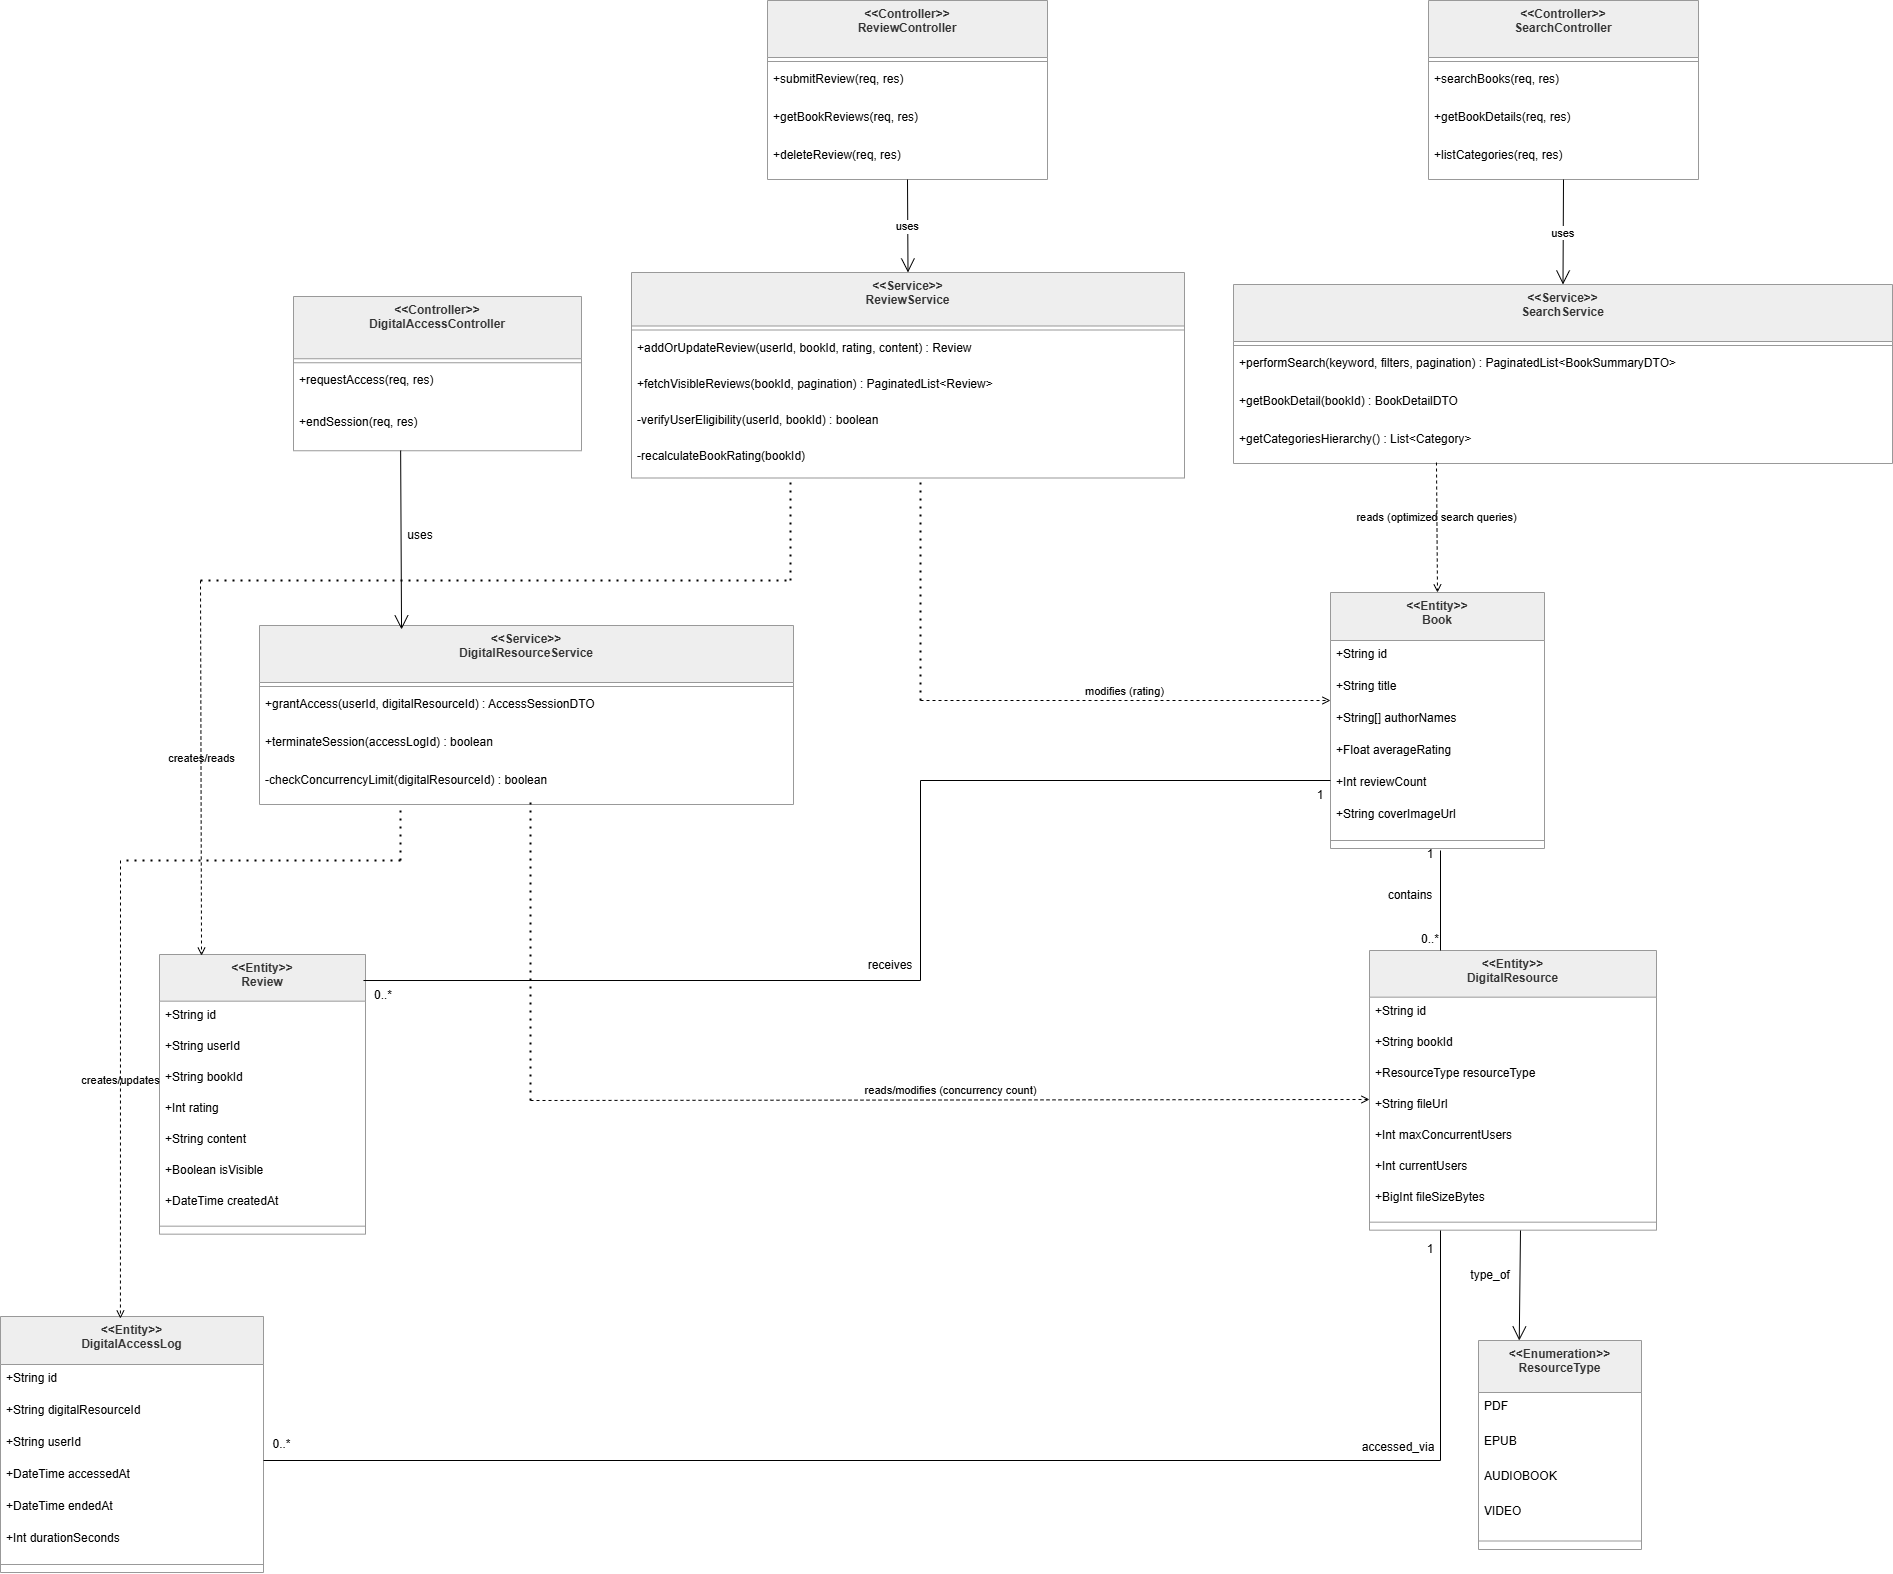
\includegraphics[width=0.6\linewidth]{Images/truycapvakhaithactainguyen.png}
	\vspace{10pt}
	\caption{Sơ đồ Lớp cho Tìm kiếm và Khai thác Tài nguyên}
	\label{fig:class_exploration}
\end{figure}

\texttt{Book} liên kết $1 - 0..*$ với \texttt{Review} ($0..* - 1$ với \texttt{Book}) lưu trữ đánh giá của người dùng.

\texttt{SearchController} sử dụng \texttt{SearchService} (\texttt{performSearch}, \texttt{getBookDetail}). \texttt{ReviewController} sử dụng \texttt{ReviewService} (\texttt{addOrUpdateReview}, \texttt{recalculateBookRating}).

\subsubsection{Trợ lý Ảo AI và Gợi ý}

\begin{figure}[H]
	\centering
	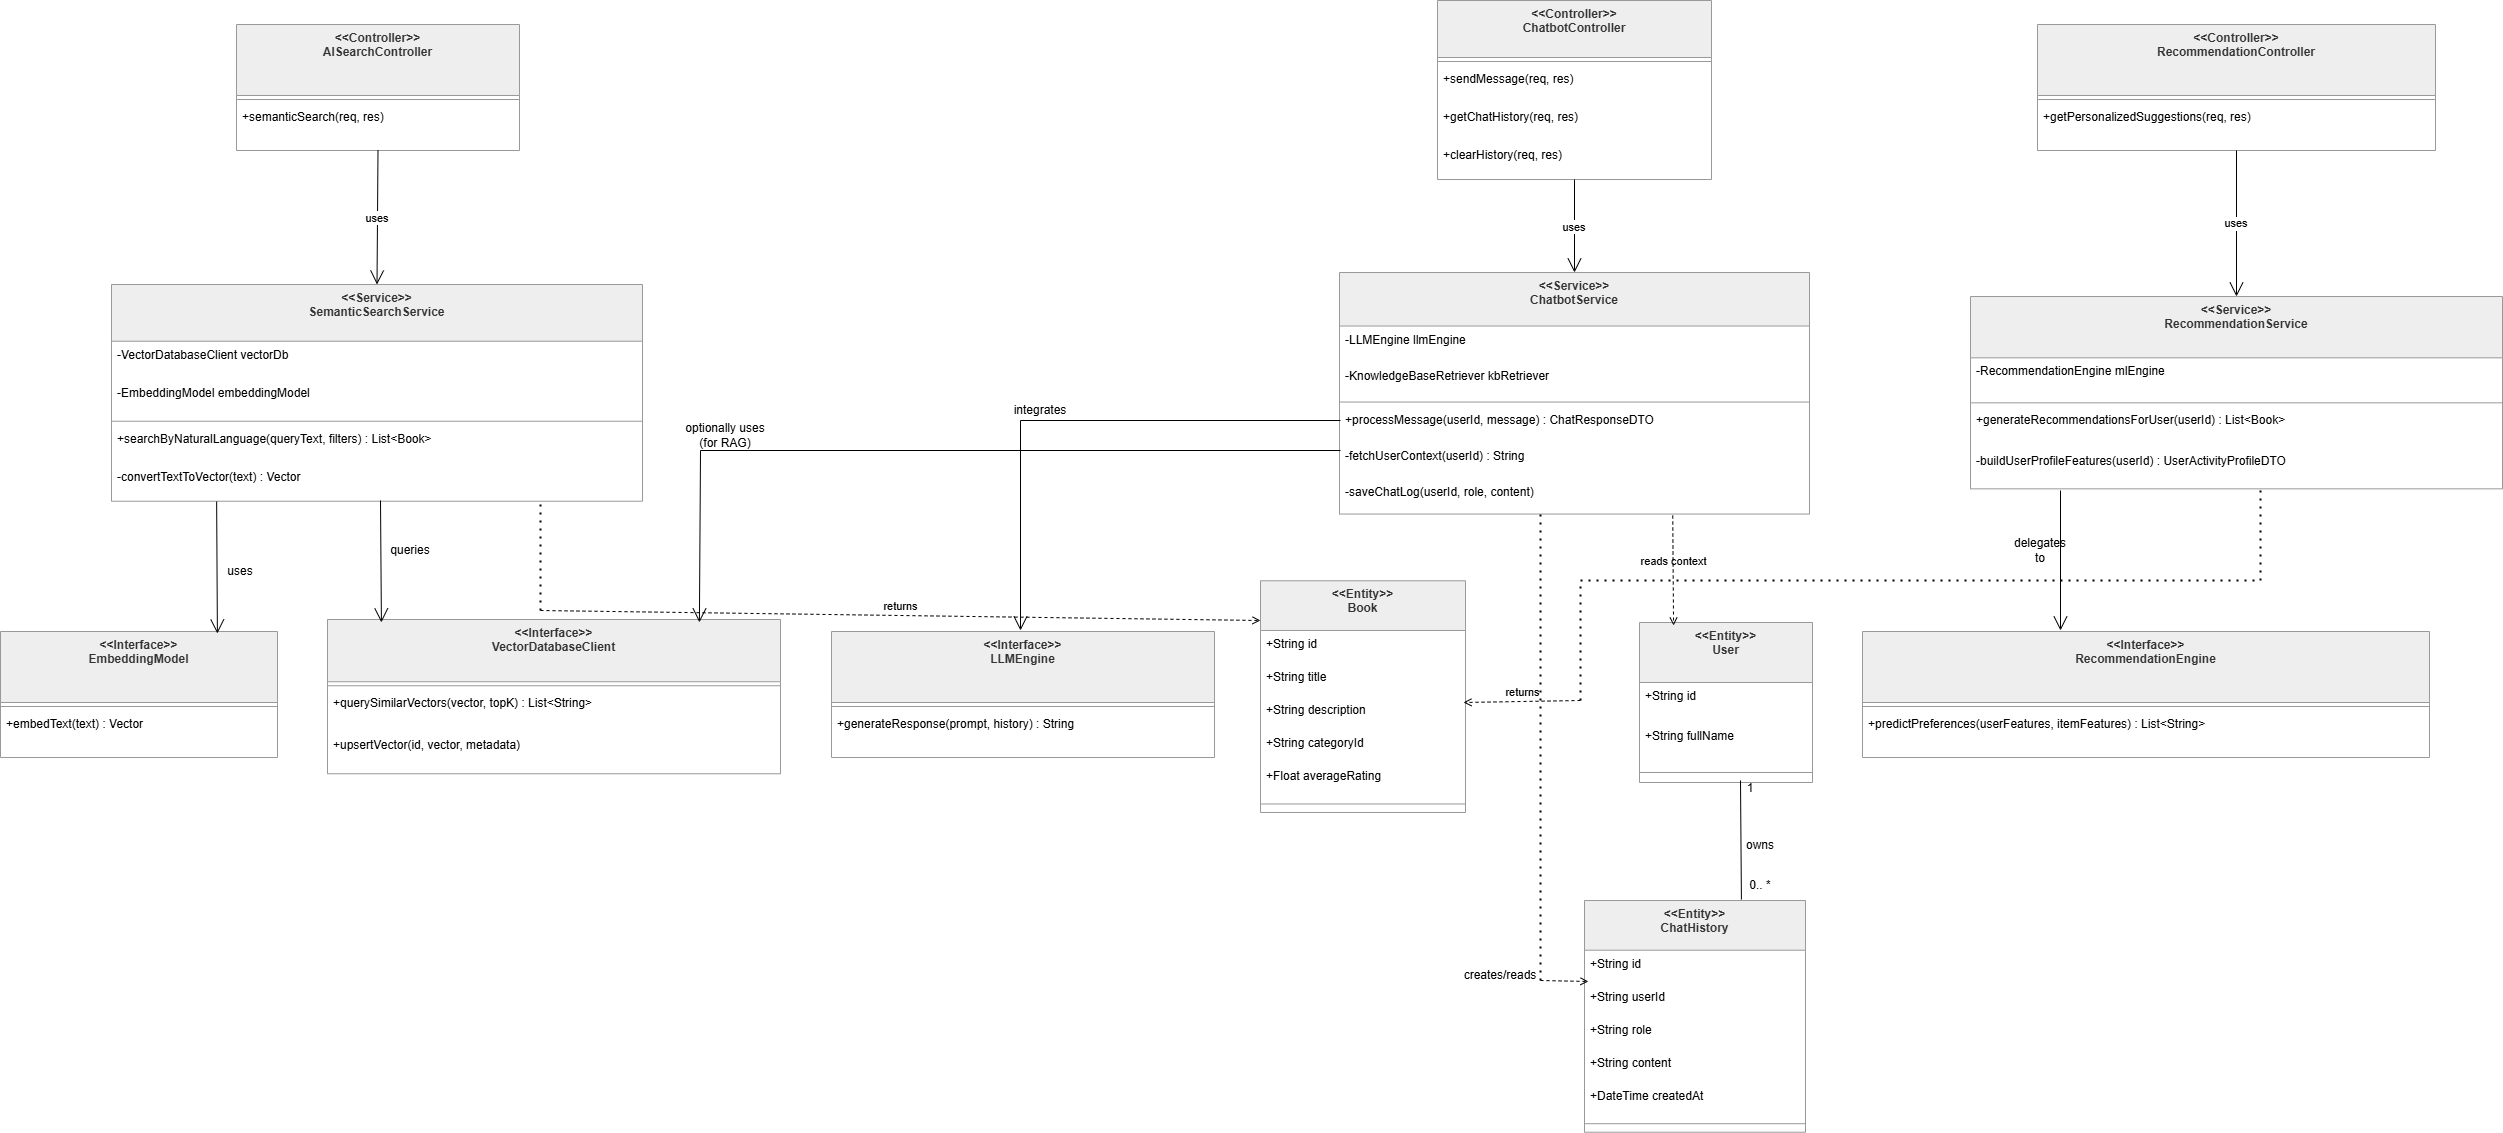
\includegraphics[width=0.6\linewidth]{Images/AI.png}
	\vspace{10pt}
	\caption{Sơ đồ Lớp cho Trợ lý Ảo AI và Gợi ý}
	\label{fig:class_ai}
\end{figure}

\texttt{AISearchController} sử dụng \texttt{SemanticSearchService} (\texttt{searchByNaturalLanguage}) giao tiếp với \texttt{EmbeddingModel} và \texttt{VectorDatabaseClient}.

\texttt{ChatbotController} sử dụng \texttt{ChatbotService} (\texttt{sendMessage}, \texttt{getChatHistory}), giao tiếp với \texttt{LLMEngine} và \texttt{VectorDatabaseClient} (ngữ cảnh RAG), ghi nhật ký hội thoại trong \texttt{ChatHistory}.

\texttt{RecommendationController} sử dụng \texttt{RecommendationService} (\texttt{getPersonalizedSuggestions}), tận dụng \texttt{RecommendationEngine} (\texttt{predictPreferences}) để trả về danh sách sách gợi ý phù hợp.

\subsubsection{Thông báo và Tương tác}

\begin{figure}[H]
	\centering
	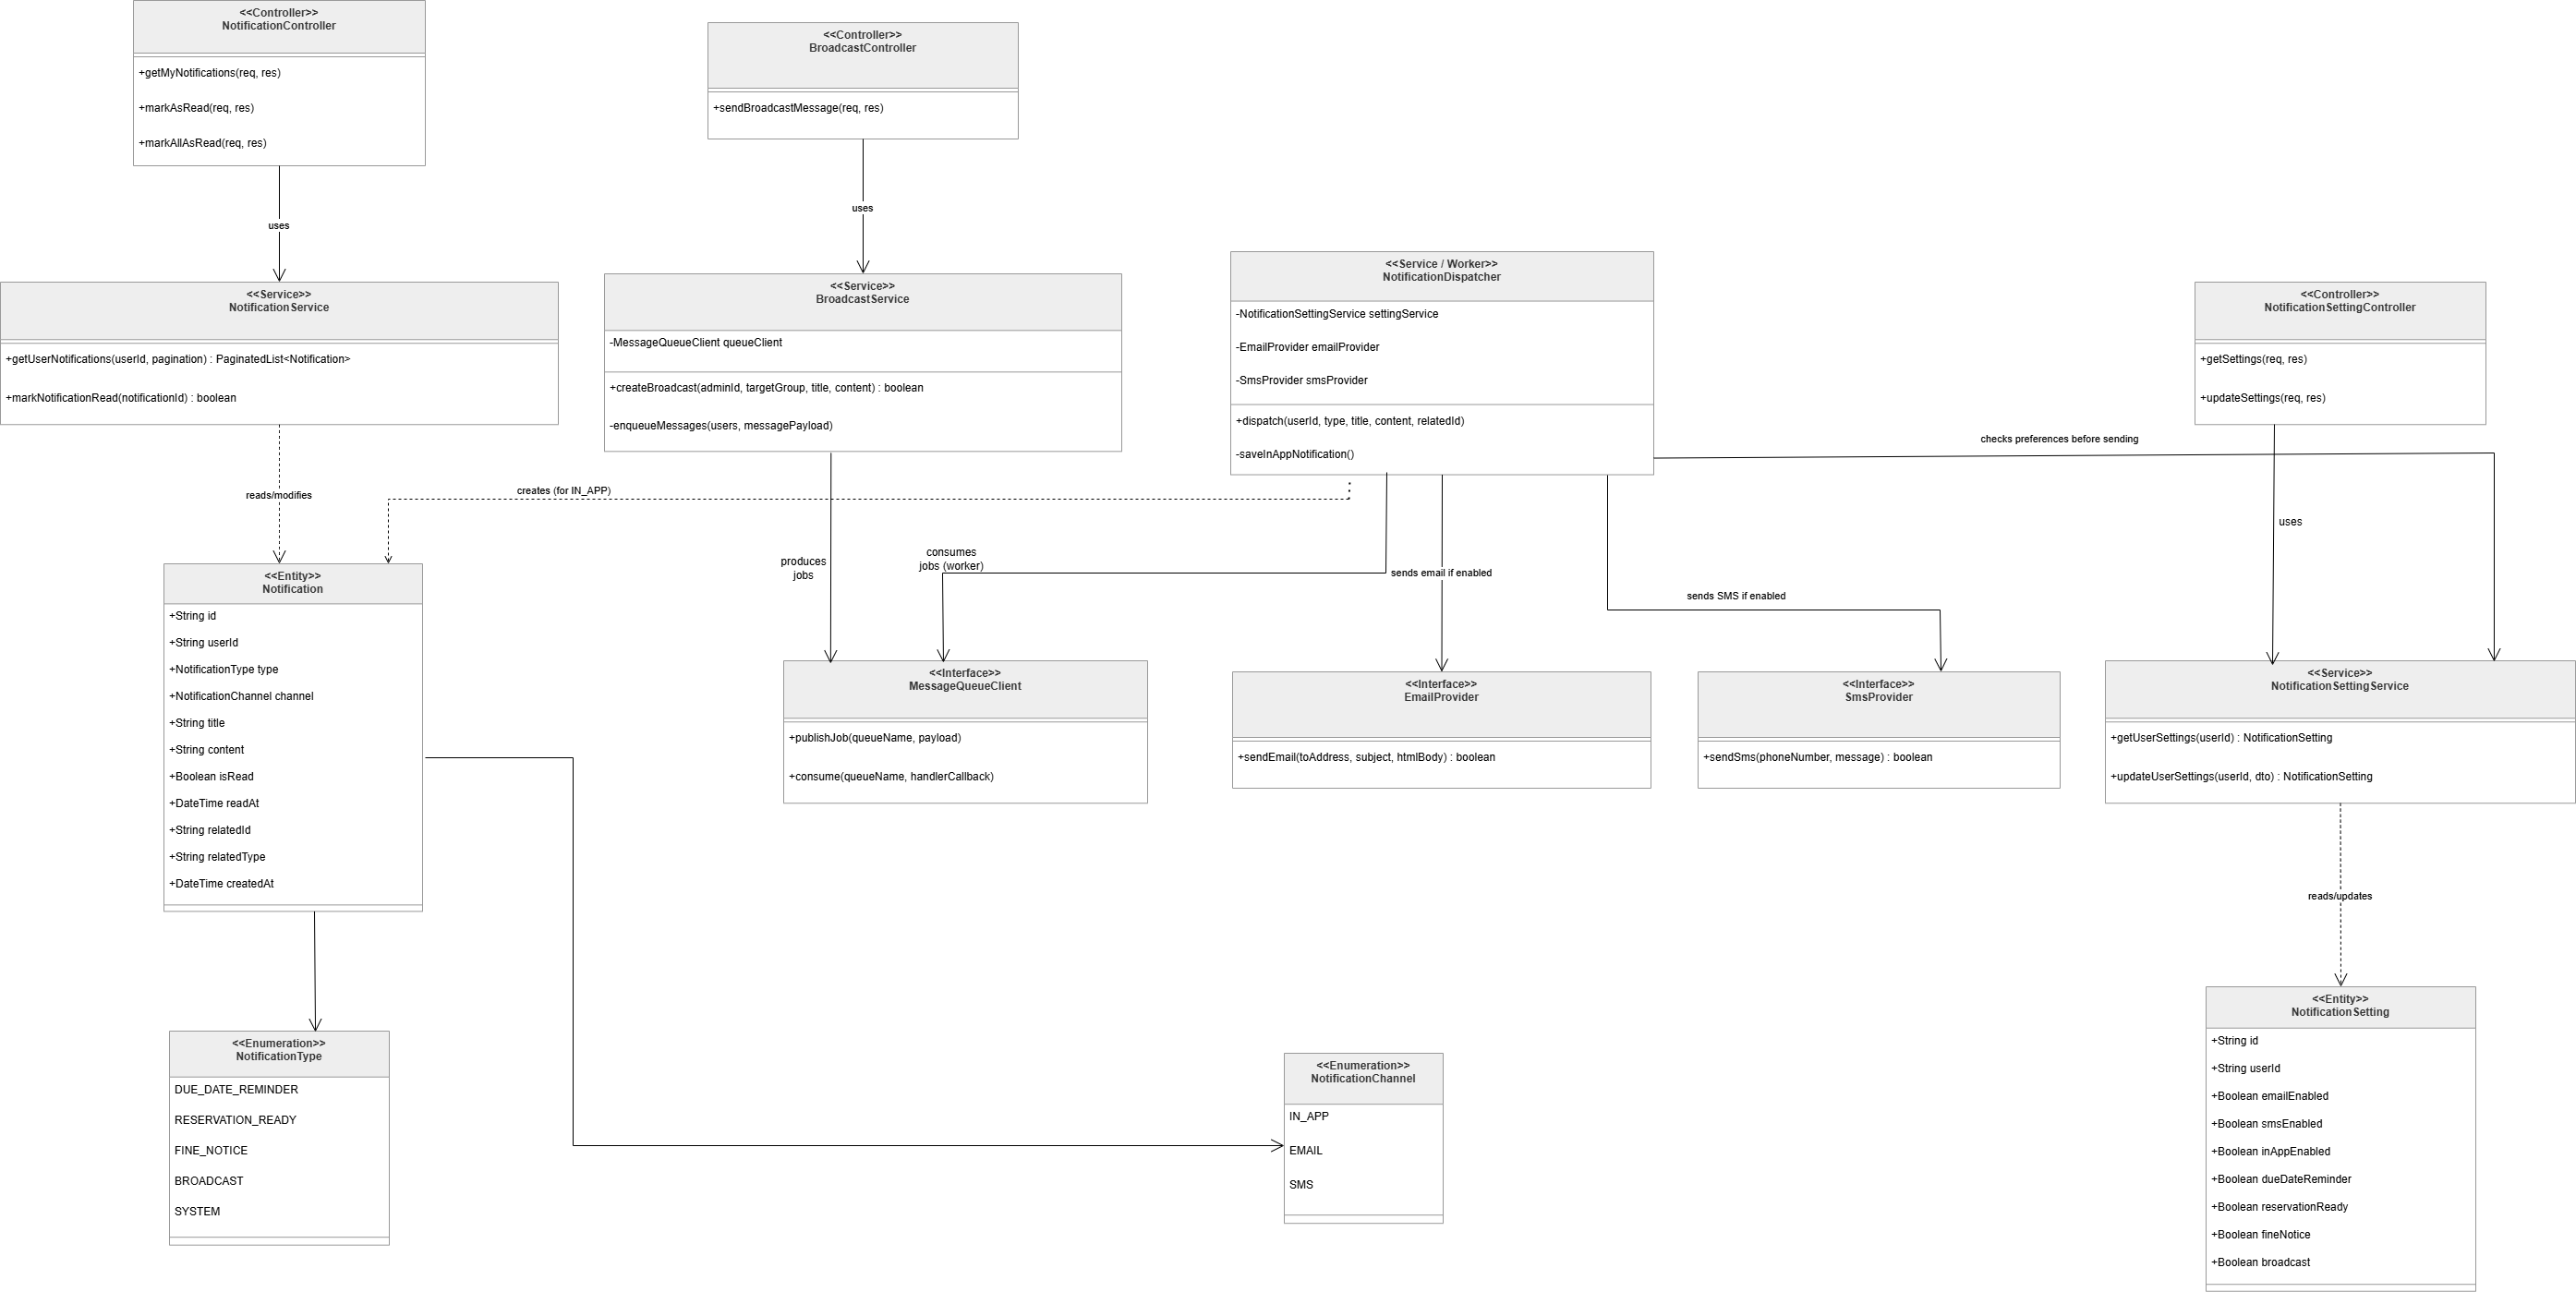
\includegraphics[width=0.6\linewidth]{Images/thongbao.png}
	\vspace{10pt}
	\caption{Sơ đồ Lớp cho Thông báo và Tương tác}
	\label{fig:class_notification}
\end{figure}

Các thực thể bao gồm \texttt{Notification} (\texttt{isRead}, \texttt{NotificationType}, \texttt{NotificationChannel}) và \texttt{NotificationSetting} (\texttt{emailEnabled}, \texttt{smsEnabled}, \texttt{inAppEnabled}).

\texttt{NotificationSettingController} sử dụng \texttt{NotificationSettingService}. \texttt{NotificationController} sử dụng \texttt{NotificationService}. \texttt{BroadcastController} sử dụng \texttt{BroadcastService} đẩy các tác vụ vào \texttt{MessageQueueClient}. Tiến trình chạy ngầm bất đồng bộ \texttt{NotificationDispatcher} xử lý các tác vụ trong hàng chờ và gửi cảnh báo qua \texttt{EmailProvider} và \texttt{SmsProvider}.

\subsubsection{Quản trị Hệ thống}

\begin{figure}[H]
	\centering
	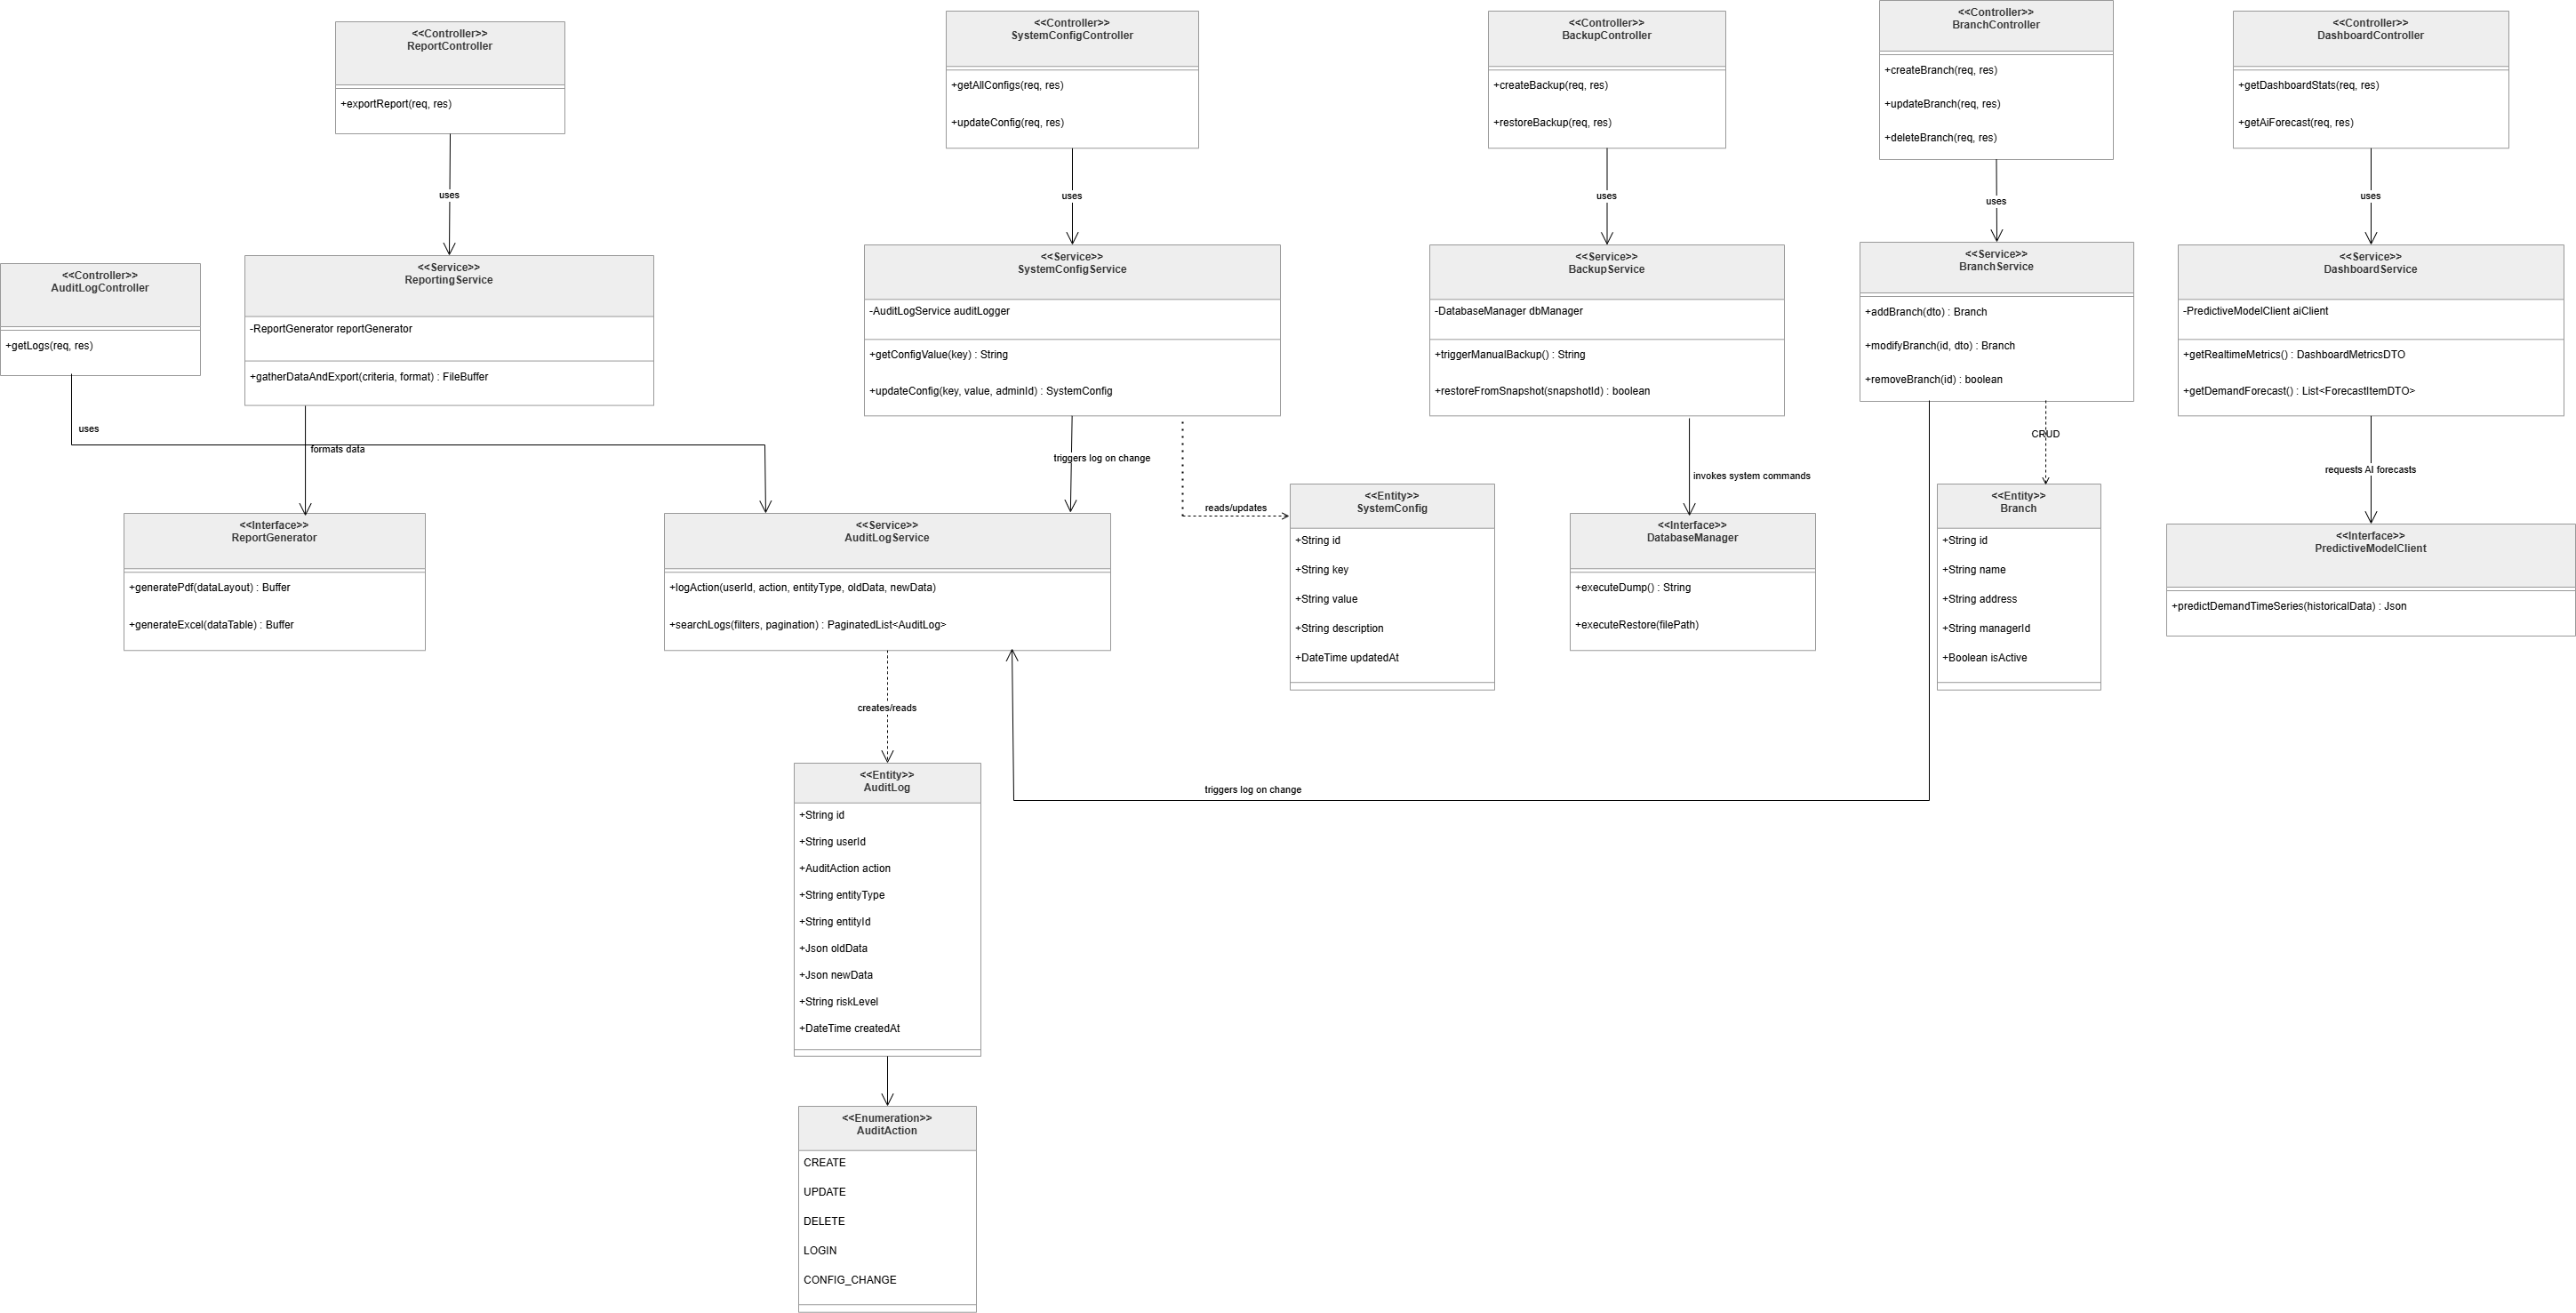
\includegraphics[width=0.6\linewidth]{Images/baocaovaquantri.png}
	\vspace{10pt}
	\caption{Sơ đồ Lớp cho Quản trị Hệ thống}
	\label{fig:class_admin}
\end{figure}

Các thực thể cốt lõi: \texttt{AuditLog} (\texttt{action}, \texttt{oldData}, \texttt{newData}, \texttt{riskLevel}), \texttt{SystemConfig} (\texttt{key}, \texttt{value}) và \texttt{Branch} (\texttt{name}, \texttt{address}, \texttt{isActive}).

\texttt{AuditLogController} sử dụng \texttt{AuditLogService}. \texttt{ReportController} sử dụng \texttt{ReportingService} (\texttt{ReportGenerator}). \texttt{SystemConfigController} sử dụng \texttt{SystemConfigService}. \texttt{BackupController} sử dụng \texttt{BackupService} (\texttt{DatabaseManager}). \texttt{BranchController} sử dụng \texttt{BranchService}. \texttt{DashboardController} sử dụng \texttt{DashboardService} giao tiếp với \texttt{PredictiveModelClient} cho dự báo nhu cầu.

\subsection{Sơ đồ Hoạt động (Activity Diagrams)}
\subsubsection{Đăng ký Tài khoản}

\begin{figure}[H]
	\centering
	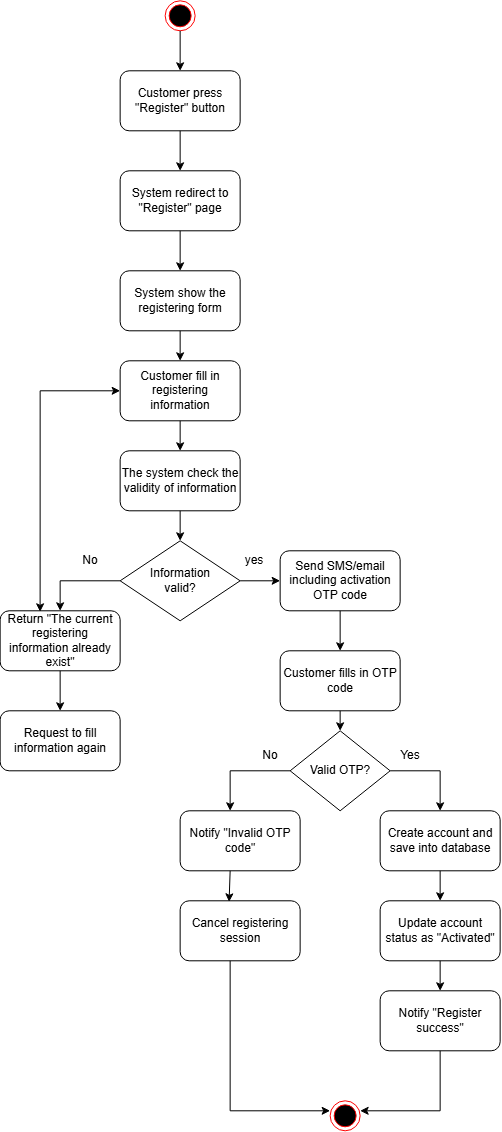
\includegraphics[width=0.6\linewidth]{Images/dangki.png}
	\vspace{10pt}
	\caption{Sơ đồ Hoạt động cho Đăng ký Tài khoản}
	\label{fig:activity_register}
\end{figure}

\begin{enumerate}
	\item Khách truy cập trang đăng ký tài khoản.
	\item Hệ thống hiển thị biểu mẫu đăng ký.
	\item Khách nhập các thông tin (Họ tên, Email/Số điện thoại, Mật khẩu).
	\item Hệ thống kiểm tra cú pháp dữ liệu đầu vào.
	\item Hệ thống kiểm tra xem Email/Số điện thoại đã tồn tại trong cơ sở dữ liệu chưa.
	\item \textbf{Nhánh Hợp lệ:}
	      \begin{itemize}
		      \item Nếu hợp lệ, hệ thống gửi Email/SMS chứa mã OTP hoặc liên kết kích hoạt.
		      \item Khách nhập mã OTP hoặc nhấn liên kết kích hoạt.
		      \item Hệ thống xác thực mã OTP hoặc token liên kết.
		      \item Nếu OTP/liên kết hợp lệ: Hệ thống tạo tài khoản người dùng, lưu vào DB, chuyển trạng thái sang "Đã kích hoạt" và báo thành công.
	      \end{itemize}
	\item \textbf{Nhánh Không Hợp lệ:}
	      \begin{itemize}
		      \item Nếu dữ liệu không hợp lệ hoặc Email/Số điện thoại đã tồn tại: Hệ thống hiển thị thông báo lỗi và yêu cầu nhập lại.
		      \item Nếu OTP không hợp lệ: Hệ thống hiển thị lỗi sai OTP và hủy phiên đăng ký.
	      \end{itemize}
\end{enumerate}

\subsubsection{Đăng nhập Hệ thống}

\begin{figure}[H]
	\centering
	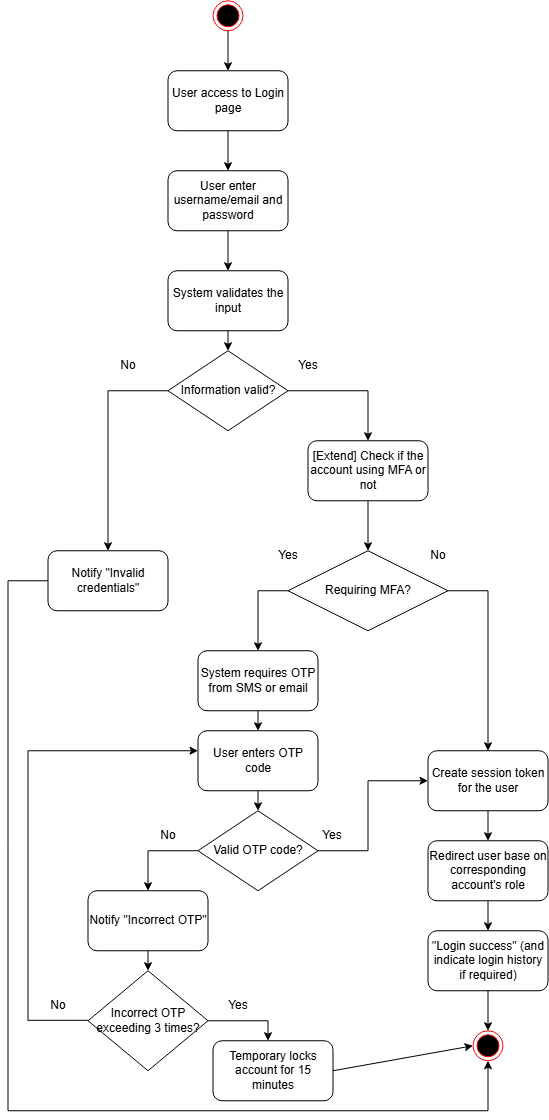
\includegraphics[width=0.6\linewidth]{Images/dangnhap.png}
	\vspace{10pt}
	\caption{Sơ đồ Hoạt động cho Đăng nhập Hệ thống}
	\label{fig:activity_login}
\end{figure}

\begin{enumerate}
	\item Người dùng truy cập giao diện đăng nhập.
	\item Người dùng nhập Email/Tên đăng nhập và Mật khẩu.
	\item Hệ thống xác thực thông tin đăng nhập với DB.
	\item Nếu thông tin không chính xác: Hệ thống hiển thị lỗi "Tài khoản hoặc mật khẩu không đúng".
	\item Nếu thông tin chính xác: Hệ thống kiểm tra xem có yêu cầu Xác thực Nhiều yếu tố (MFA) hay không.
	\item Nếu bật MFA: Hệ thống yêu cầu mã OTP; người dùng nhập OTP; hệ thống xác thực mã.
	\item Nếu OTP sai: Hiển thị lỗi "Mã OTP không chính xác". Nếu nhập sai quá 3 lần, tài khoản bị tạm khóa trong 15 phút.
	\item Nếu OTP đúng (hoặc không yêu cầu MFA): Khởi tạo phiên/token, chuyển hướng người dùng đến bảng điều khiển theo vai trò và hiển thị thông báo thành công.
\end{enumerate}

\subsubsection{Đặt lại Mật khẩu}

\begin{figure}[H]
	\centering
	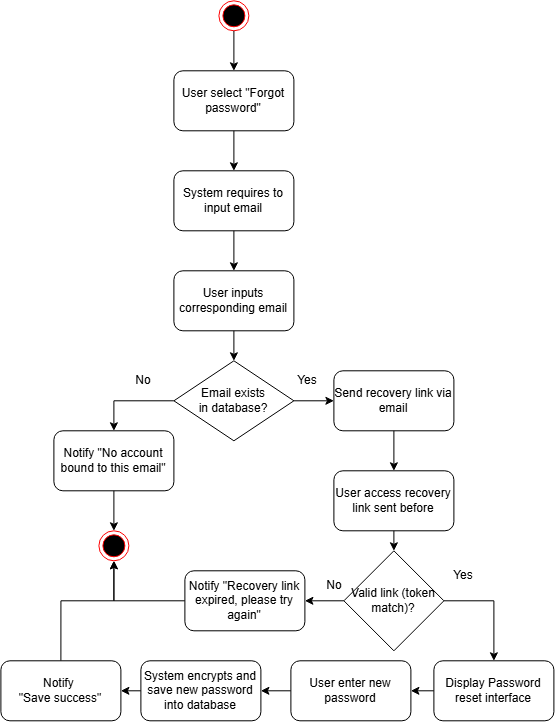
\includegraphics[width=0.6\linewidth]{Images/datlai.png}
	\vspace{10pt}
	\caption{Sơ đồ Hoạt động cho Đặt lại Mật khẩu}
	\label{fig:activity_reset_password}
\end{figure}

\begin{enumerate}
	\item Người dùng chọn "Quên mật khẩu".
	\item Hệ thống yêu cầu nhập Email.
	\item Người dùng gửi Email.
	\item Hệ thống xác minh sự tồn tại của Email. Nếu không tìm thấy: Hiển thị "Không tìm thấy tài khoản với email này".
	\item Nếu tìm thấy: Hệ thống gửi liên kết đặt lại qua Email. Người dùng mở liên kết; hệ thống kiểm tra tính hợp lệ của token.
	\item Nếu liên kết hết hạn/không hợp lệ: Hiển thị "Liên kết đặt lại đã hết hạn" và yêu cầu thực hiện lại.
	\item Nếu liên kết hợp lệ: Hiển thị biểu mẫu đặt lại; người dùng nhập mật khẩu mới; hệ thống băm và cập nhật mật khẩu, thông báo thành công.
\end{enumerate}

\subsubsection{Xem Lịch sử Mượn/Trả}

\begin{figure}[H]
	\centering
	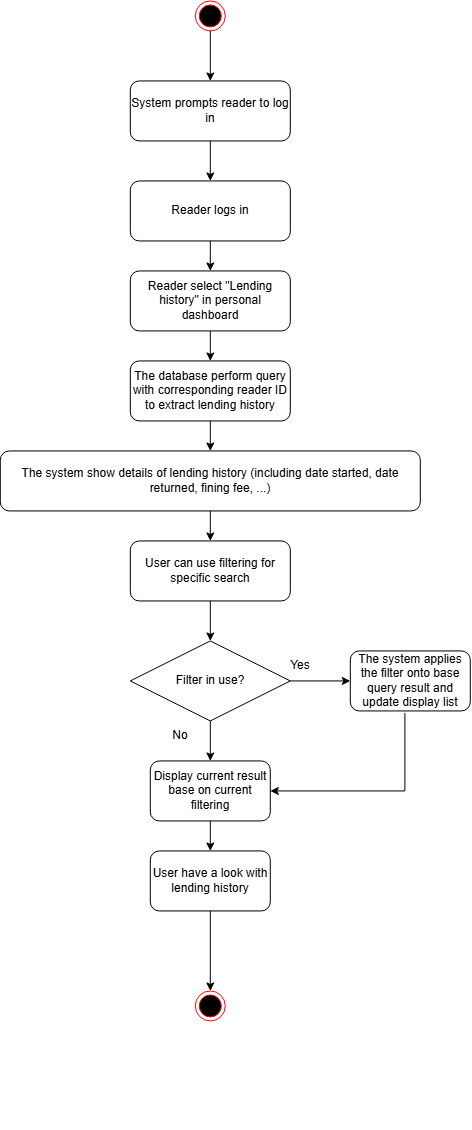
\includegraphics[width=0.6\linewidth]{Images/xemlichsu.png}
	\vspace{10pt}
	\caption{Sơ đồ Hoạt động cho Xem Lịch sử Mượn/Trả}
	\label{fig:activity_view_history}
\end{figure}

\begin{enumerate}
	\item Người dùng đăng nhập vào hệ thống.
	\item Người dùng mở "Lịch sử Mượn trả" trên bảng điều khiển.
	\item Hệ thống truy vấn DB lấy các bản ghi mượn khớp với ID Người dùng.
	\item Hệ thống hiển thị bảng lịch sử mượn (Tên sách, Ngày mượn, Hạn trả, Ngày trả, Trạng thái, Tiền phạt).
	\item Người dùng có thể áp dụng bộ lọc theo khoảng thời gian hoặc trạng thái.
	\item Hệ thống làm mới bảng hiển thị dựa trên tham số lọc.
\end{enumerate}

\subsubsection{Quản lý Tài khoản Người dùng}

\begin{figure}[H]
	\centering
	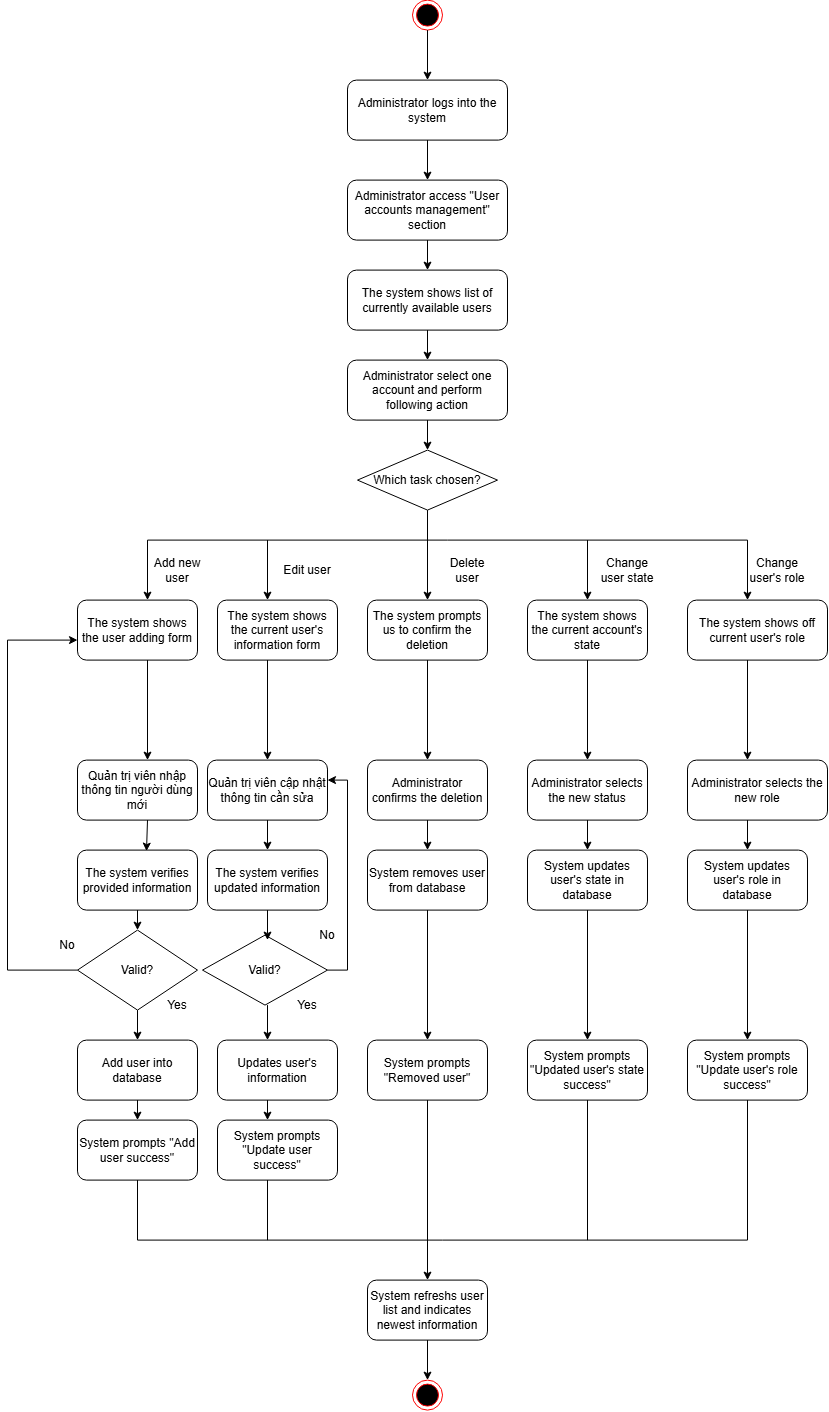
\includegraphics[width=0.6\linewidth]{Images/quanly.png}
	\vspace{10pt}
	\caption{Sơ đồ Hoạt động cho Quản lý Tài khoản Người dùng}
	\label{fig:activity_manage_users}
\end{figure}

\begin{enumerate}
	\item Admin đăng nhập và truy cập "Quản lý Người dùng".
	\item Hệ thống hiển thị danh sách người dùng (ID, Tên, Email, Vai trò, Trạng thái).
	\item Admin chọn người dùng đích và một thao tác (Thêm người dùng, Sửa hồ sơ, Xóa người dùng, Chuyển trạng thái, Thay đổi vai trò).
	\item Thực hiện quy trình đã chọn; hệ thống kiểm tra dữ liệu đầu vào và cập nhật DB, hiển thị thông báo thành công khi hoàn tất.
\end{enumerate}

\subsubsection{Thêm / Sửa / Xóa Bản ghi Danh mục}

\begin{figure}[H]
	\centering
	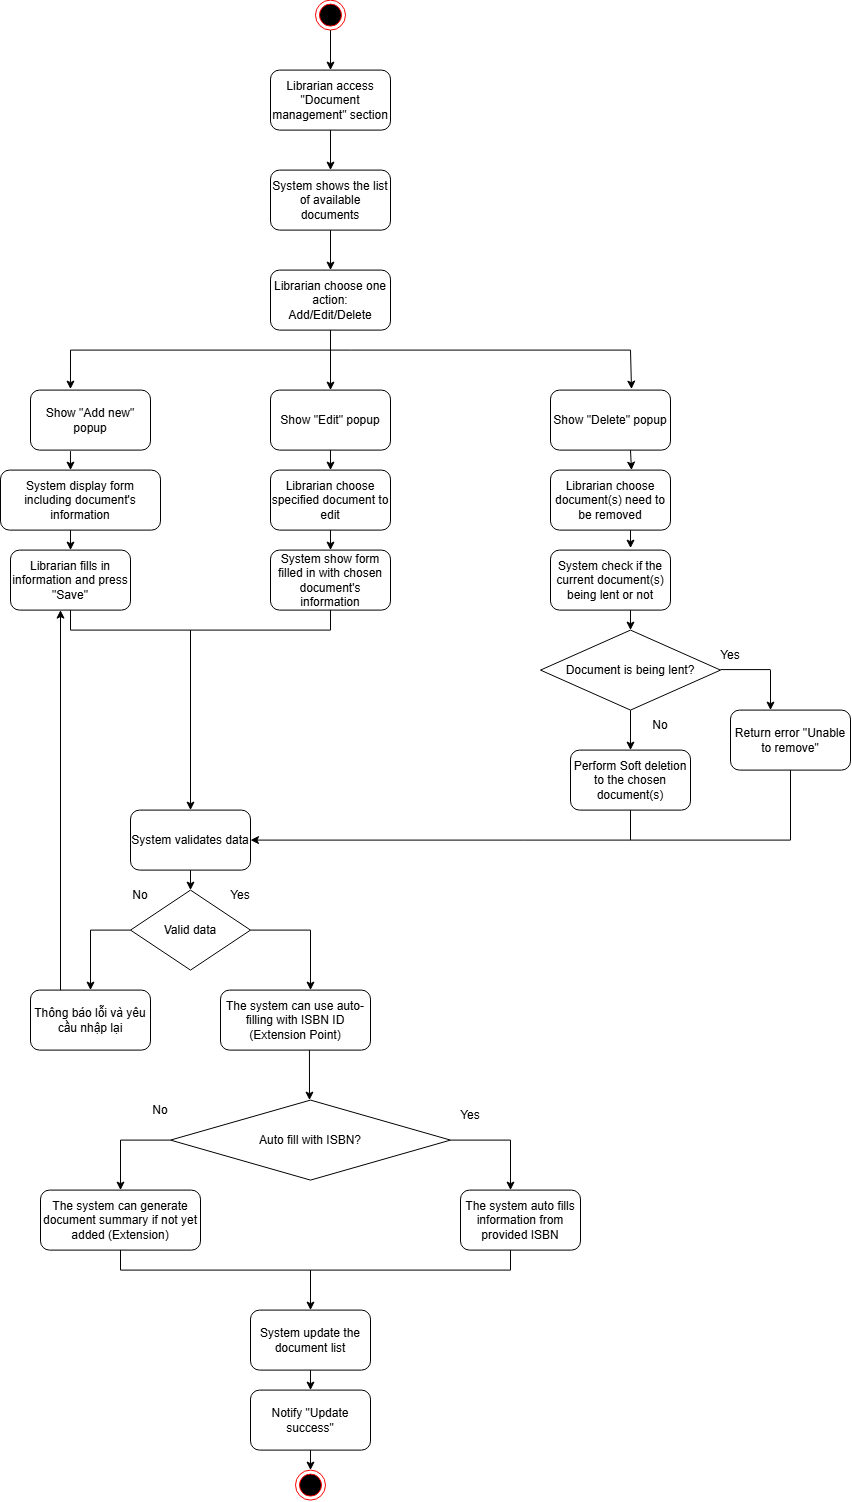
\includegraphics[width=0.6\linewidth]{Images/edit.png}
	\vspace{10pt}
	\caption{Sơ đồ Hoạt động cho Thêm / Sửa / Xóa Bản ghi Danh mục}
	\label{fig:activity_manage_documents}
\end{figure}

\begin{enumerate}
	\item Thủ thư mở "Quản lý Danh mục".
	\item Thủ thư chọn thao tác: Thêm, Sửa, hoặc Xóa.
	\item Nếu Xóa: Hệ thống kiểm tra các bản mượn đang hoạt động. Nếu tài liệu đang được mượn, chặn xóa ("Không thể xóa: Tài liệu đang được mượn"). Nguợc lại, thực hiện xóa mềm (Soft Delete).
	\item Nếu Thêm/Sửa: Biểu mẫu được hiển thị; có thể kích hoạt tùy chọn tự động biên mục qua ISBN (UC-CAT-03) hoặc tạo tóm tắt AI (UC-CAT-04).
	\item Hệ thống kiểm tra các trường, lưu cập nhật và báo thành công.
\end{enumerate}

\subsubsection{Nhập Dữ liệu Danh mục Hàng loạt}

\begin{figure}[H]
	\centering
	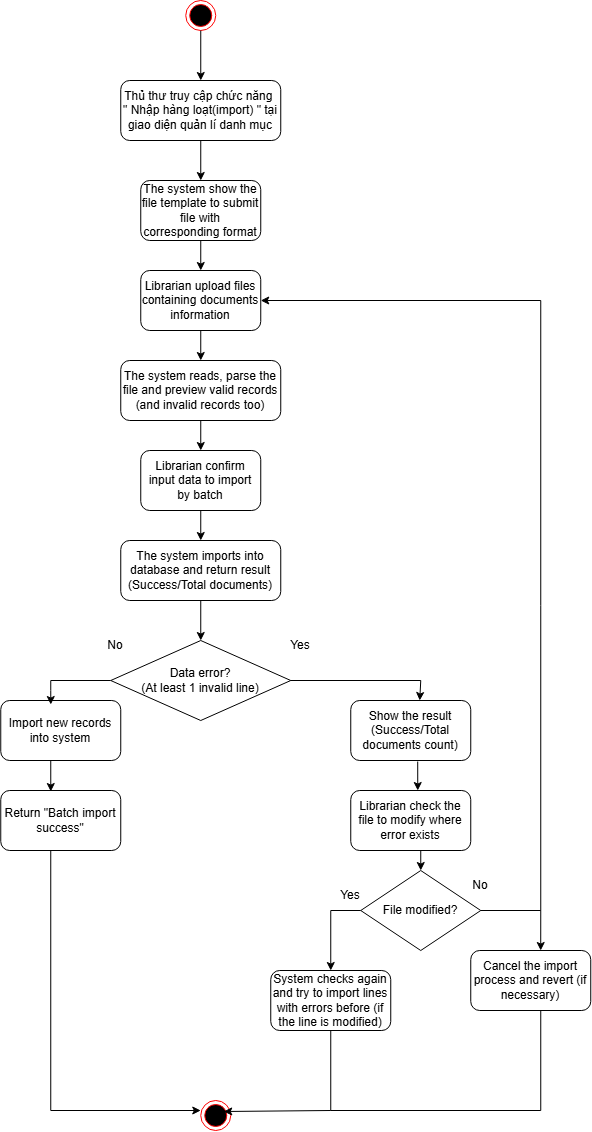
\includegraphics[width=0.6\linewidth]{Images/nhap.png}
	\vspace{10pt}
	\caption{Sơ đồ Hoạt động cho Nhập Dữ liệu Danh mục Hàng loạt}
	\label{fig:activity_import}
\end{figure}

\begin{enumerate}
	\item Thủ thư chọn "Nhập Hàng loạt".
	\item Tải lên tệp dữ liệu danh mục (CSV/Excel).
	\item Hệ thống đọc tệp và hiển thị bảng xem trước với số lượng bản ghi hợp lệ/không hợp lệ.
	\item Thủ thư xác nhận thực hiện nhập.
	\item Hệ thống ghi các dòng hợp lệ vào DB và báo cáo kết quả. Nếu có lỗi, thủ thư có thể sửa tệp và tải lại hoặc hủy thao tác.
\end{enumerate}

\subsubsection{Biên mục Tự động qua ISBN}

\begin{figure}[H]
	\centering
	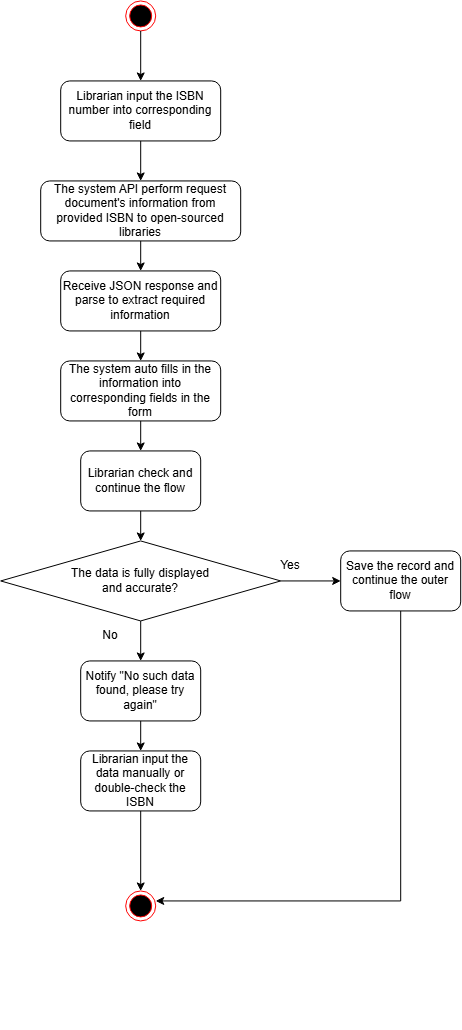
\includegraphics[width=0.6\linewidth]{Images/bienmuc.png}
	\vspace{10pt}
	\caption{Sơ đồ Hoạt động cho Biên mục Tự động qua ISBN}
	\label{fig:activity_isbn}
\end{figure}

\begin{enumerate}
	\item Thủ thư nhập mã ISBN.
	\item Hệ thống gửi yêu cầu API đến các nguồn bên ngoài (Google Books, Open Library).
	\item Phân tích phản hồi JSON và điền vào các trường biểu mẫu.
	\item Thủ thư xem lại và lưu bản ghi danh mục. Nếu không tìm thấy ISBN, thủ thư chuyển sang nhập thủ công.
\end{enumerate}

\subsubsection{Mượn Tài liệu Vật lý}

\begin{figure}[H]
	\centering
	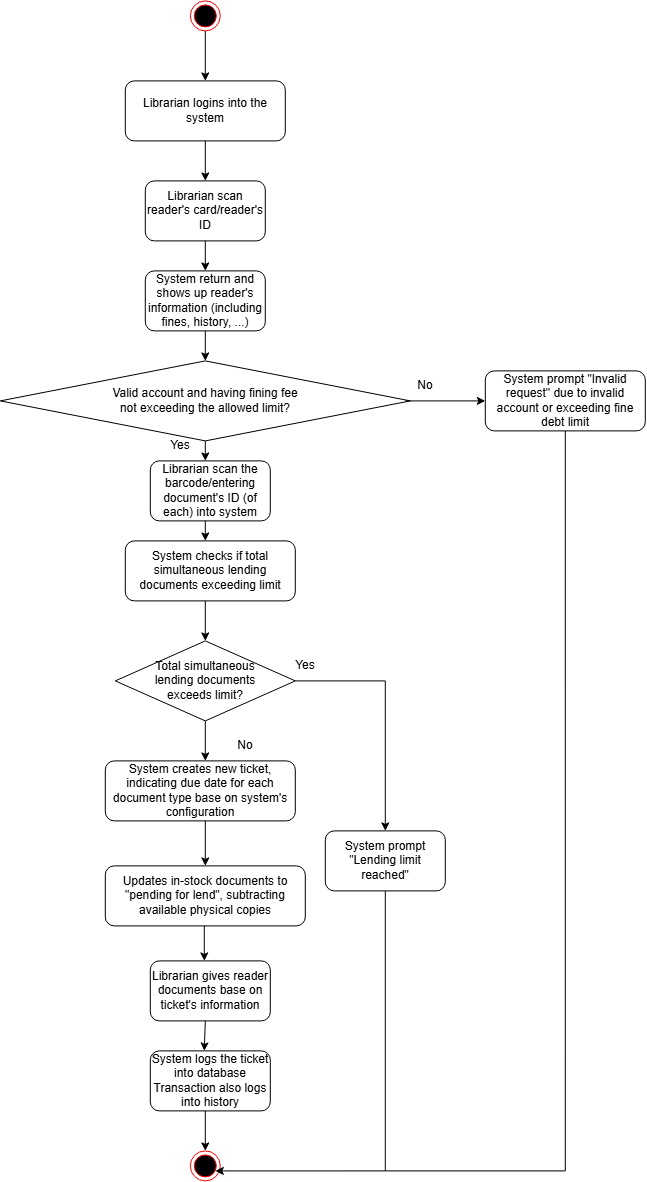
\includegraphics[width=0.6\linewidth]{Images/muon.png}
	\vspace{10pt}
	\caption{Sơ đồ Hoạt động cho Mượn Tài liệu Vật lý}
	\label{fig:activity_borrow}
\end{figure}

\begin{enumerate}
	\item Thủ thư đăng nhập và quét mã vạch thẻ Độc giả.
	\item Hệ thống kiểm tra trạng thái tài khoản và số tiền phạt chưa thanh toán.
	\item Nếu đủ điều kiện, thủ thư quét mã vạch các tài liệu mượn.
	\item Hệ thống kiểm tra hạn mức mượn theo vai trò và hạn chế từ hàng chờ đặt chỗ.
	\item Tạo bản ghi mượn, tính hạn trả, cập nhật trạng thái bản sao thành "Đã mượn" và giảm số lượng kho.
\end{enumerate}

\subsubsection{Trả Tài liệu}

\begin{figure}[H]
	\centering
	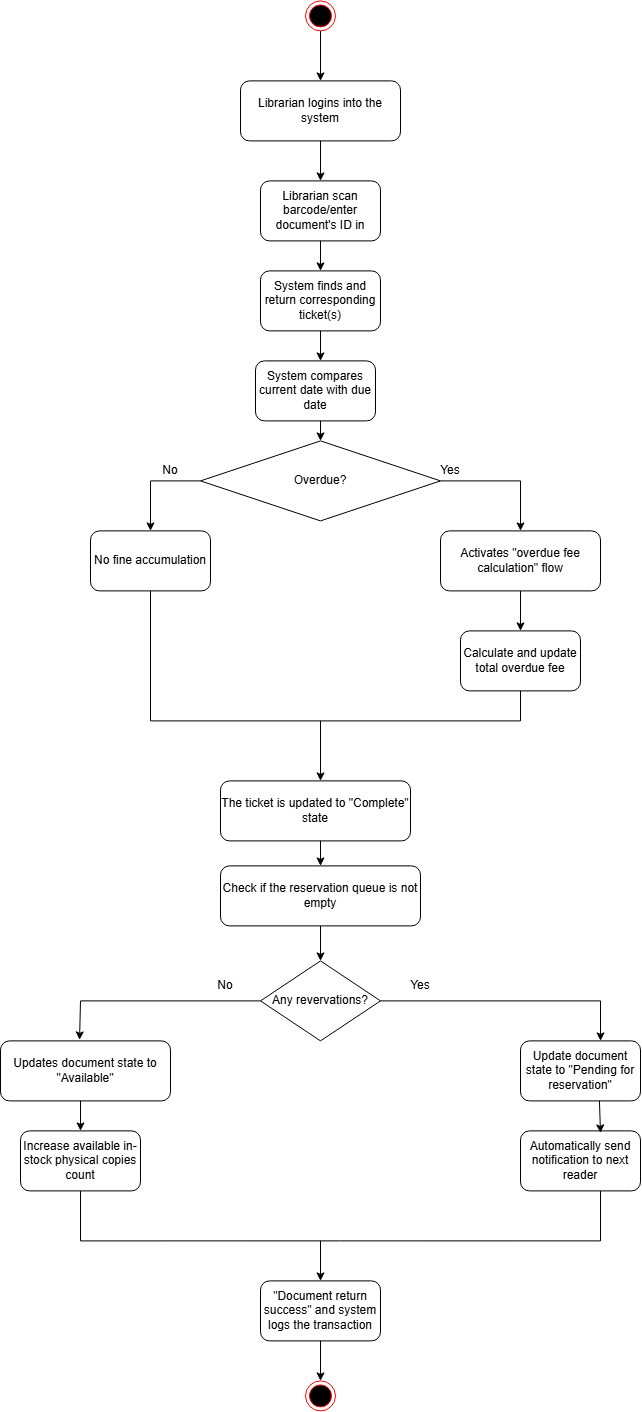
\includegraphics[width=0.6\linewidth]{Images/tra.png}
	\vspace{10pt}
	\caption{Sơ đồ Hoạt động cho Trả Tài liệu}
	\label{fig:activity_return}
\end{figure}

\begin{enumerate}
	\item Thủ thư quét mã vạch tài liệu trả.
	\item Hệ thống lấy bản ghi mượn và kiểm tra hạn trả.
	\item Nếu quá hạn, kích hoạt quy trình tính phạt (UC-CIR-03).
	\item Đặt trạng thái lượt mượn thành "Hoàn thành".
	\item Kiểm tra hàng chờ đặt chỗ: nếu có lượt đặt, đặt bản sao thành "Chờ lấy sách" và thông báo cho người dùng tiếp theo; nếu không có lượt đặt, đặt bản sao thành "Khả dụng".
\end{enumerate}

\subsubsection{Tính và Thu Phạt Quá hạn}

\begin{figure}[H]
	\centering
	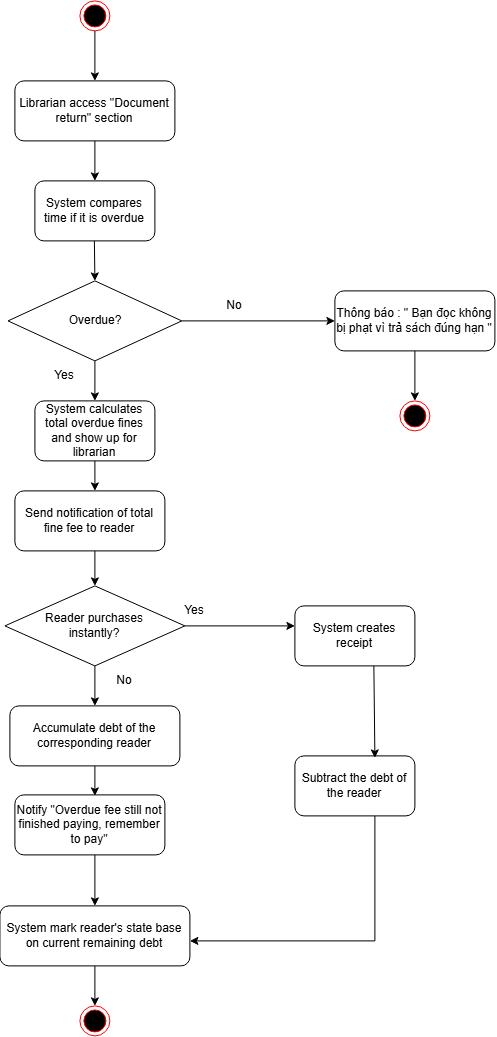
\includegraphics[width=0.5\linewidth]{Images/phiphat.png}
	\vspace{10pt}
	\caption{Sơ đồ Hoạt động cho Tính và Thu Phạt Quá hạn}
	\label{fig:activity_fine}
\end{figure}

\begin{enumerate}
	\item Hệ thống tính số ngày quá hạn (Ngày trả - Hạn trả), loại trừ các ngày lễ của thư viện.
	\item Nhân số ngày quá hạn với mức phí phạt hằng ngày.
	\item Hiển thị khoản phạt tính toán. Nếu độc giả thanh toán ngay, xuất hóa đơn và đặt số dư phạt về 0; ngược lại ghi khoản phạt vào sổ nợ tài khoản độc giả.
\end{enumerate}

\subsubsection{Gia hạn Mượn Trực tuyến}

\begin{figure}[H]
	\centering
	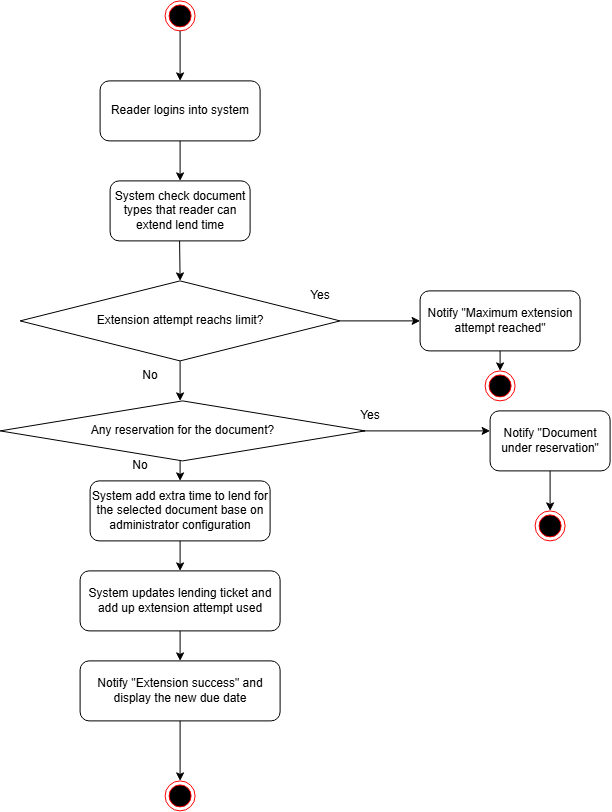
\includegraphics[width=0.6\linewidth]{Images/giahan.png}
	\vspace{10pt}
	\caption{Sơ đồ Hoạt động cho Gia hạn Mượn Trực tuyến}
	\label{fig:activity_extend}
\end{figure}

\begin{enumerate}
	\item Độc giả mở danh sách mượn hiện tại và nhấn "Gia hạn".
	\item Hệ thống kiểm tra: chưa vượt quá số lần gia hạn tối đa và không có yêu cầu đặt chỗ nào khác.
	\item Nếu đủ điều kiện, kéo dài hạn trả, tăng số lần gia hạn và hiển thị hạn trả mới.
\end{enumerate}

\subsubsection{Đặt Giữ chỗ Tài liệu}

\begin{figure}[H]
	\centering
	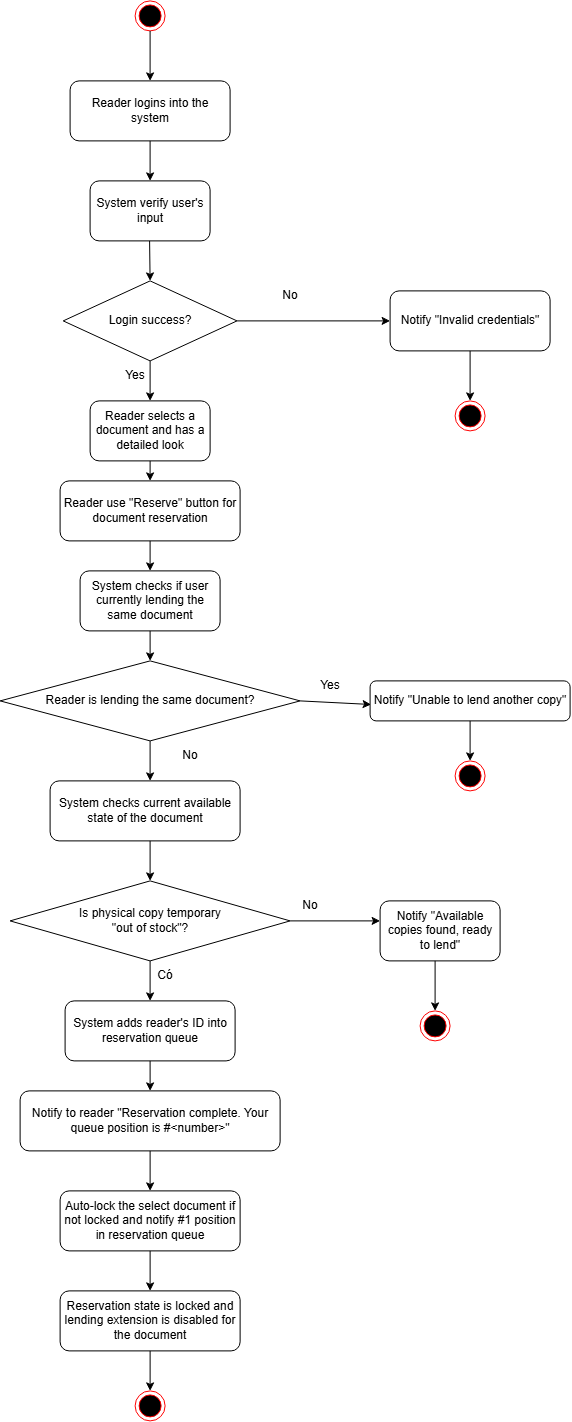
\includegraphics[width=0.5\linewidth]{Images/dat.png}
	\vspace{10pt}
	\caption{Sơ đồ Hoạt động cho Đặt Giữ chỗ Tài liệu}
	\label{fig:activity_reserve}
\end{figure}

\begin{enumerate}
	\item Độc giả mở trang chi tiết tài liệu và nhấn "Đặt chỗ".
	\item Hệ thống kiểm tra độc giả hiện không mượn tài liệu này và tất cả các bản sao đều đã được mượn hết.
	\item Hệ thống thêm độc giả vào hàng chờ đặt chỗ và hiển thị vị trí trong hàng chờ.
\end{enumerate}

\subsubsection{Tìm kiếm Danh mục Tài liệu}

\begin{figure}[H]
	\centering
	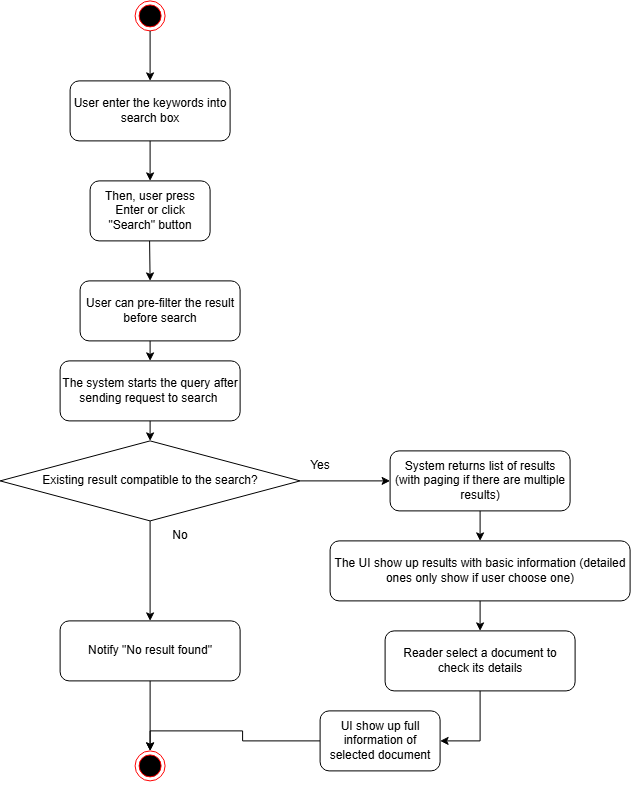
\includegraphics[width=0.6\linewidth]{Images/tracuu.png}
	\vspace{10pt}
	\caption{Sơ đồ Hoạt động cho Tìm kiếm Danh mục Tài liệu}
	\label{fig:activity_search}
\end{figure}

\begin{enumerate}
	\item Độc giả nhập từ khóa tìm kiếm và chọn tiêu chí tra cứu.
	\item Hệ thống truy vấn các chỉ mục cơ sở dữ liệu danh mục và trả về kết quả phân trang.
	\item Hiển thị thẻ sách. Độc giả nhấn vào thẻ sách để xem trang chi tiết.
\end{enumerate}

\subsection{Sơ đồ Tuần tự (Sequence Diagrams)}

\subsubsection{Đăng ký Tài khoản}
\begin{figure}[H]
	\centering
	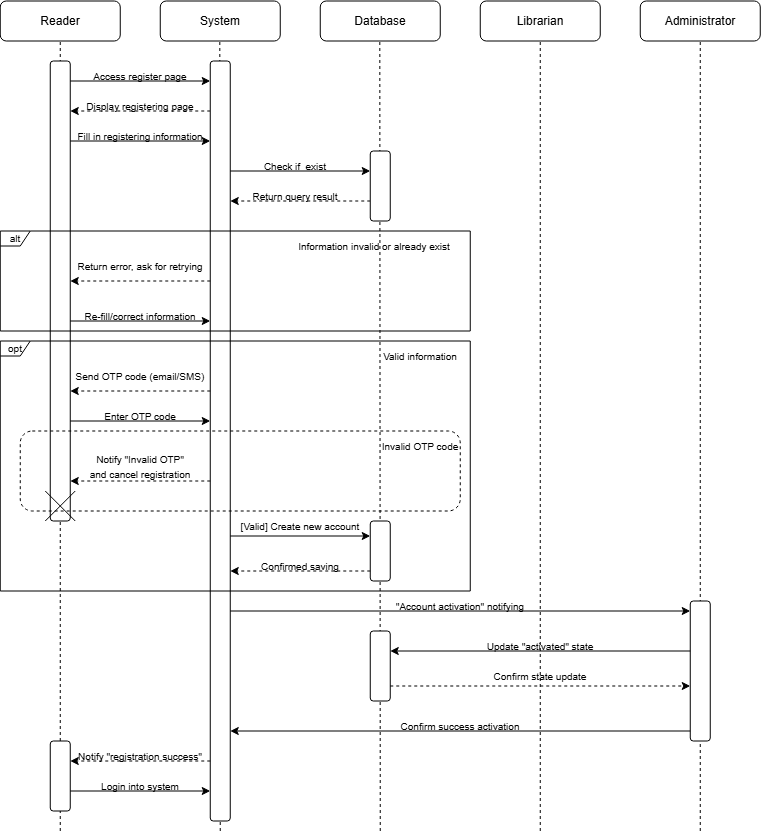
\includegraphics[width=0.6\linewidth]{Images/Seq_Dang ky.png}
	\vspace{10pt}
	\caption{Sơ đồ Tuần tự cho Đăng ký Tài khoản}
	\label{fig:sequence_register}
\end{figure}
\begin{enumerate}
	\item Độc giả truy cập giao diện đăng ký.
	\item Gửi thông tin; hệ thống kiểm tra dữ liệu và trùng lặp.
	\item Hệ thống gửi mã OTP qua email/SMS.
	\item Độc giả nhập OTP. Nếu OTP hợp lệ, tài khoản được tạo và kích hoạt; ngược lại quá trình đăng ký bị hủy.
\end{enumerate}

\subsubsection{Đăng nhập Hệ thống}
\begin{figure}[H]
	\centering
	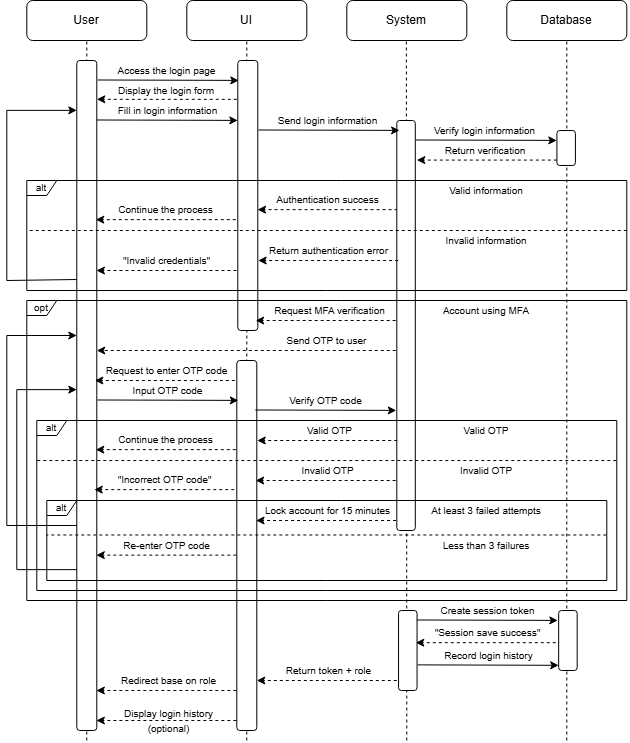
\includegraphics[width=0.6\linewidth]{Images/Seq_Dang nhap.png}
	\vspace{10pt}
	\caption{Sơ đồ Tuần tự cho Đăng nhập Hệ thống}
	\label{fig:sequence_login}
\end{figure}
\begin{enumerate}
	\item Người dùng gửi thông tin đăng nhập.
	\item Hệ thống đối chiếu thông tin với DB.
	\item Nếu bật MFA, yêu cầu mã OTP; khi xác thực OTP thành công, cấp session JWT token và chuyển hướng người dùng đến bảng điều khiển theo vai trò.
\end{enumerate}

\subsubsection{Đặt lại Mật khẩu Tài khoản}
\begin{figure}[H]
	\centering
	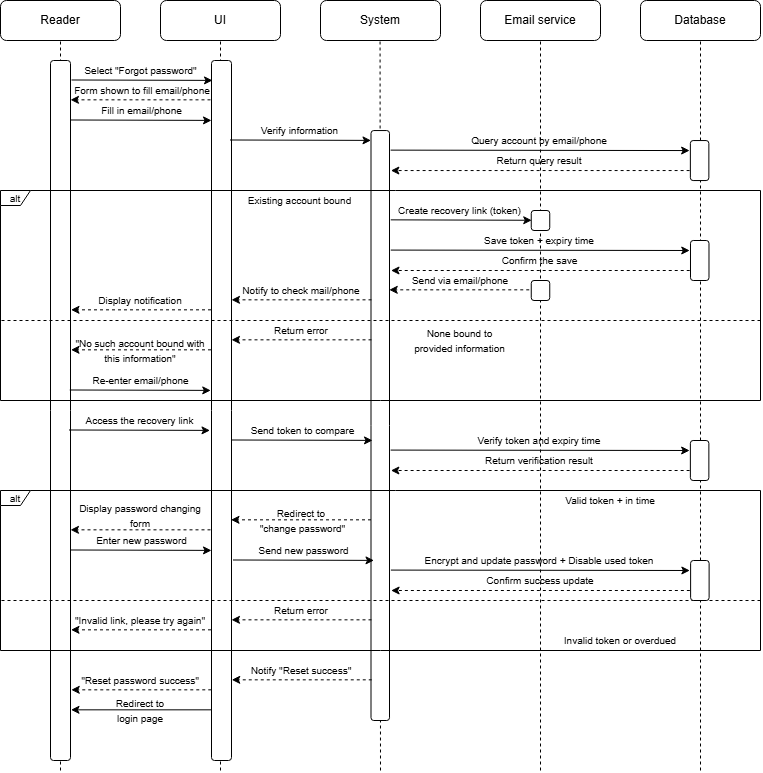
\includegraphics[width=0.6\linewidth]{Images/Seq_Reset mat khau.png}
	\vspace{10pt}
	\caption{Sơ đồ Tuần tự cho Đặt lại Mật khẩu Tài khoản}
	\label{fig:sequence_reset_password}
\end{figure}
\begin{enumerate}
	\item Người dùng yêu cầu đặt lại mật khẩu bằng cách nhập email đã đăng ký.
	\item Hệ thống xác minh email, tạo reset token và gửi liên kết đặt lại qua email.
	\item Người dùng mở liên kết; hệ thống xác thực token. Người dùng gửi mật khẩu mới; hệ thống cập nhật băm mật khẩu.
\end{enumerate}

\subsubsection{Tìm kiếm Tài liệu}
\begin{figure}[H]
	\centering
	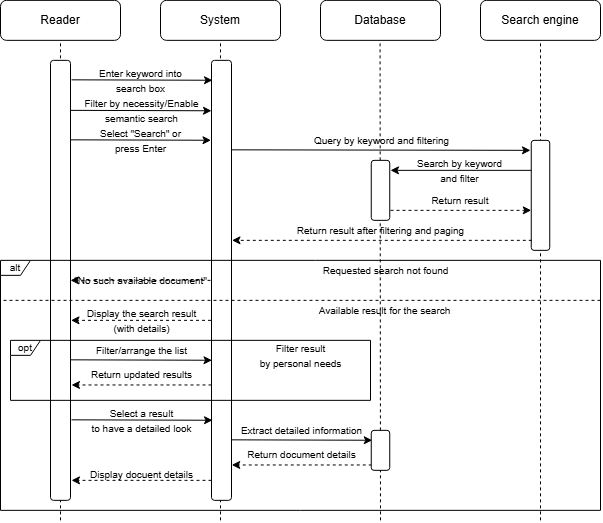
\includegraphics[width=0.6\linewidth]{Images/Seq_Tim kiem.png}
	\vspace{10pt}
	\caption{Sơ đồ Tuần tự cho Tìm kiếm Tài liệu}
	\label{fig:sequence_search}
\end{figure}
\begin{enumerate}
	\item Độc giả nhập câu truy vấn tìm kiếm.
	\item Công cụ tìm kiếm truy vấn cơ sở dữ liệu danh mục và trả về kết quả đã lọc và phân trang.
	\item Hiển thị các thẻ tài liệu; nhấn vào tài liệu để lấy bản ghi chi tiết.
\end{enumerate}

\subsubsection{Thêm / Sửa / Xóa Tài liệu}
\subsubsubsection{Thêm Tài liệu}
\begin{figure}[H]
	\centering
	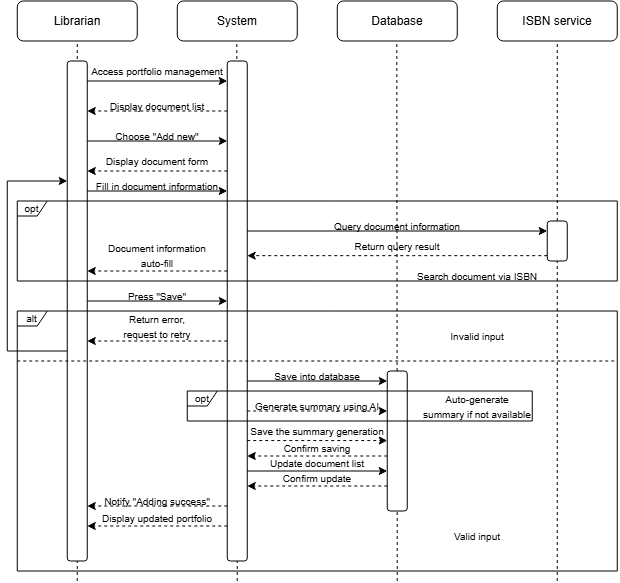
\includegraphics[width=0.6\linewidth]{Images/Seq_Them tai lieu.png}
	\vspace{10pt}
	\caption{Sơ đồ Tuần tự cho Thêm Tài liệu}
	\label{fig:sequence_add_document}
\end{figure}
Thủ thư nhập dữ liệu tả thủ công hoặc lấy qua ISBN API (UC-CAT-03), có thể tạo tóm tắt AI (UC-CAT-04), và lưu bản ghi.

\subsubsubsection{Sửa Tài liệu}
\begin{figure}[H]
	\centering
	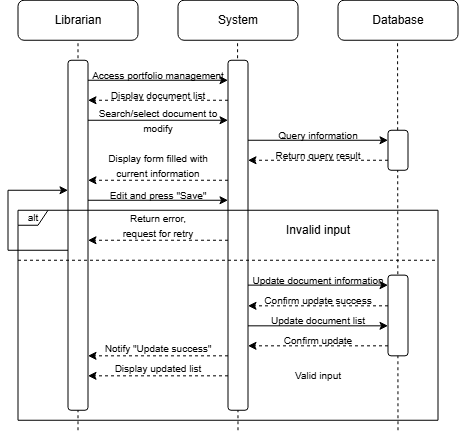
\includegraphics[width=0.6\linewidth]{Images/Seq_Sua tai lieu.png}
	\vspace{10pt}
	\caption{Sơ đồ Tuần tự cho Sửa Tài liệu}
	\label{fig:sequence_edit_document}
\end{figure}
Thủ thư chỉnh sửa các trường tài liệu đã điền sẵn, hệ thống kiểm tra dữ liệu đầu vào và cập nhật bản ghi DB.

\subsubsubsection{Xóa Tài liệu}
\begin{figure}[H]
	\centering
	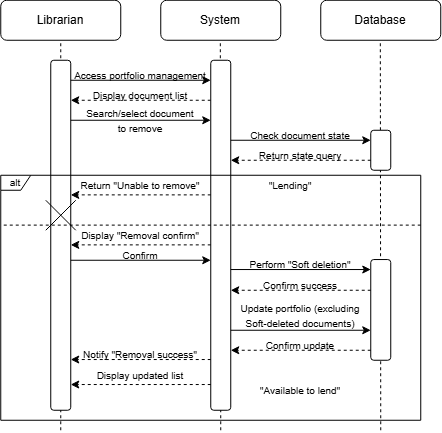
\includegraphics[width=0.6\linewidth]{Images/Seq_Xoa tai lieu.png}
	\vspace{10pt}
	\caption{Sơ đồ Tuần tự cho Xóa Tài liệu}
	\label{fig:sequence_delete_document}
\end{figure}
Hệ thống xác minh tài liệu hiện không được mượn, thủ thư xác nhận xóa và hệ thống thực hiện xóa mềm.

\subsubsection{Nhập Tài liệu Hàng loạt}
\begin{figure}[H]
	\centering
	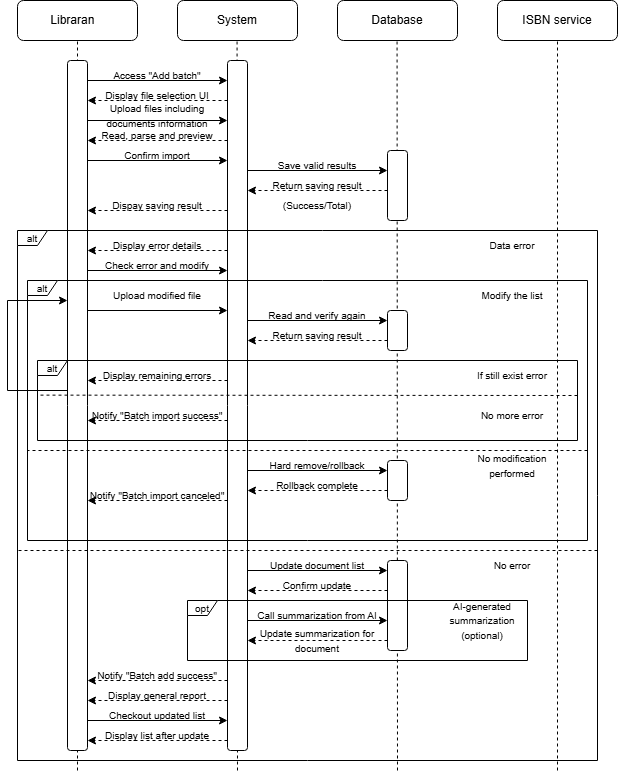
\includegraphics[width=0.6\linewidth]{Images/Seq_Them hang loat.png}
	\vspace{10pt}
	\caption{Sơ đồ Tuần tự cho Nhập Tài liệu Hàng loạt}
	\label{fig:sequence_import_documents}
\end{figure}
Thủ thư tải tệp lên; hệ thống kiểm tra các dòng, nhập các dòng hợp lệ và báo cáo tổng hợp lỗi.

\subsubsection{Đặt Giữ chỗ Tài liệu}
\begin{figure}[H]
	\centering
	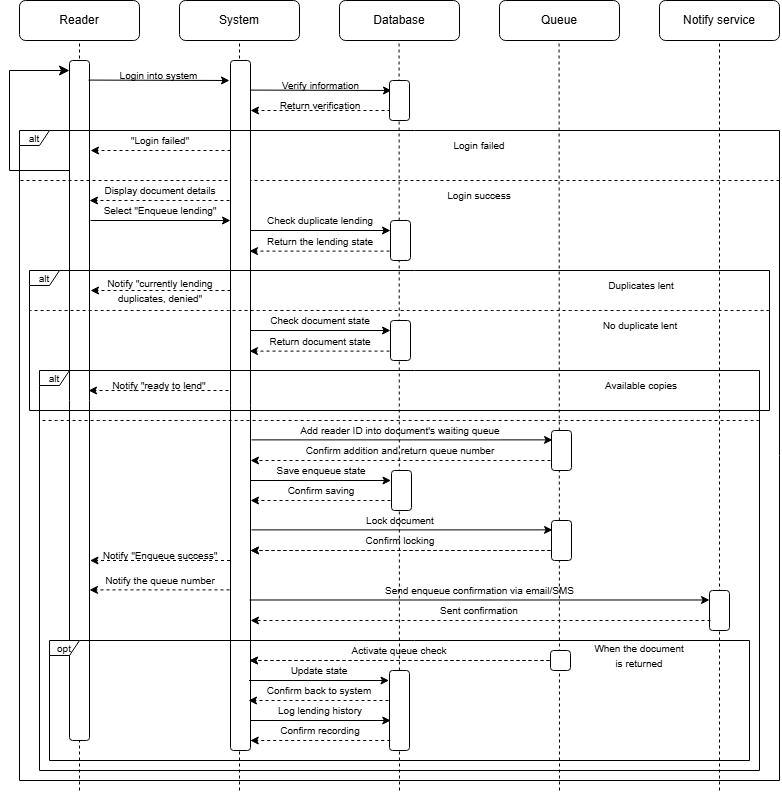
\includegraphics[width=0.6\linewidth]{Images/Seq_Dat muon sach.png}
	\vspace{10pt}
	\caption{Sơ đồ Tuần tự cho Đặt Giữ chỗ Tài liệu}
	\label{fig:sequence_reserve_document}
\end{figure}
Hệ thống kiểm tra trùng lặp lượt mượn và tình trạng bản sao khả dụng; nếu không còn bản sao khả dụng nào, thêm người dùng vào hàng chờ và gửi email xác nhận.

\subsubsection{Cập nhật Tính Phạt}
\begin{figure}[H]
	\centering
	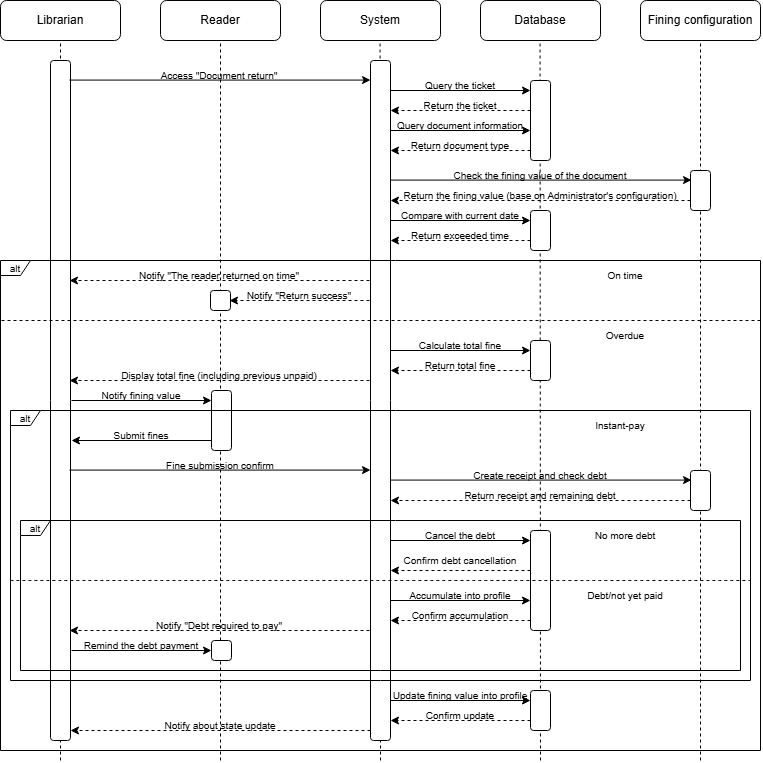
\includegraphics[width=0.6\linewidth]{Images/Seq_Tien phat.png}
	\vspace{10pt}
	\caption{Sơ đồ Tuần tự cho Cập nhật Tính Phạt}
	\label{fig:sequence_fine}
\end{figure}
Hệ thống kiểm tra ngưỡng phạt của độc giả, quét tài liệu, tạo phiếu mượn và giảm số lượng kho.

\subsubsection{Xử lý Mượn Tài liệu}
\begin{figure}[H]
	\centering
	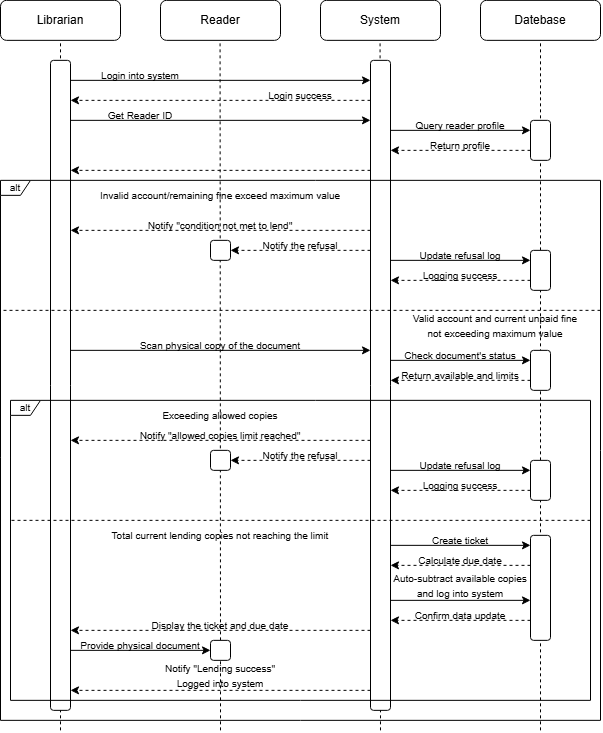
\includegraphics[width=0.6\linewidth]{Images/Seq_Muon sach.png}
	\vspace{10pt}
	\caption{Sơ đồ Tuần tự cho Xử lý Mượn Tài liệu}
	\label{fig:sequence_borrow}
\end{figure}
Thủ thư xác minh điều kiện độc giả, kiểm tra trạng thái giữ chỗ tài liệu, kiểm tra hạn mức mượn và tạo phiếu mượn.

\subsubsection{Gia hạn Mượn Tài liệu}
\begin{figure}[H]
	\centering
	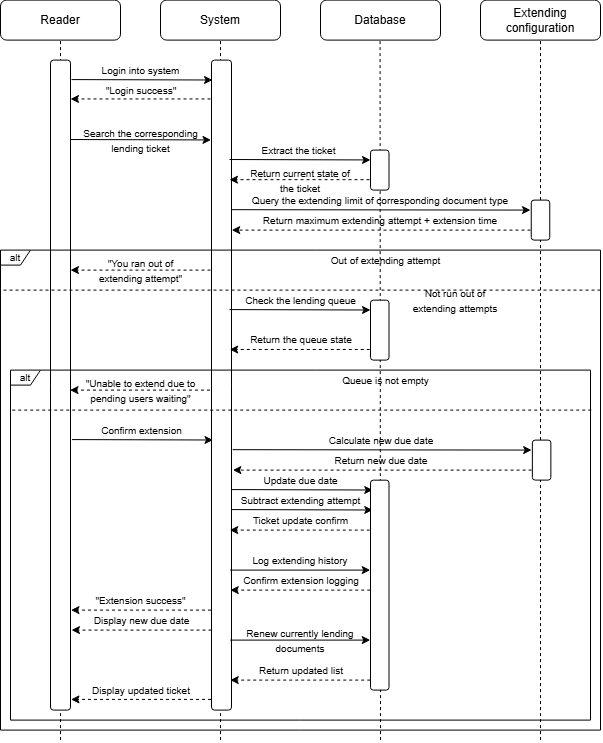
\includegraphics[width=0.6\linewidth]{Images/Seq_Gia han.png}
	\vspace{10pt}
	\caption{Sơ đồ Tuần tự cho Gia hạn Mượn Tài liệu}
	\label{fig:sequence_extend_borrow}
\end{figure}
Hệ thống kiểm tra số lần gia hạn cho phép và trạng thái hàng chờ đặt chỗ; kéo dài hạn trả khi được chấp thuận.

\subsubsection{Trả Tài liệu}
\begin{figure}[H]
	\centering
	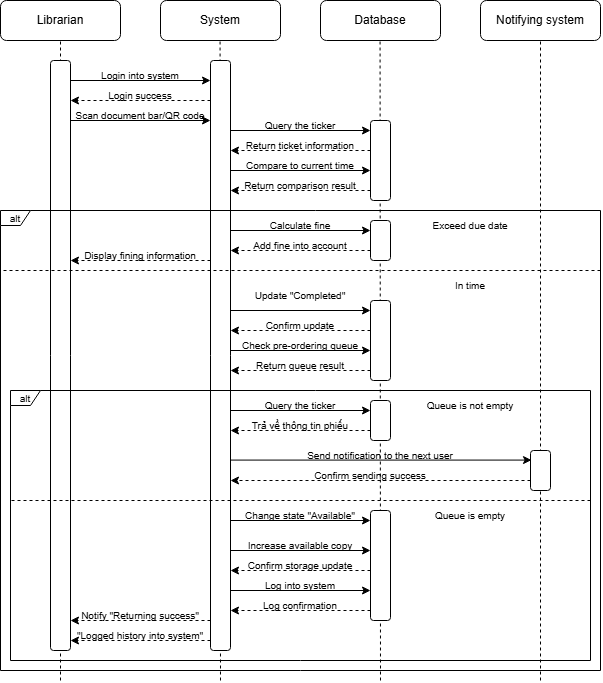
\includegraphics[width=0.6\linewidth]{Images/Seq_Tra sach.png}
	\vspace{10pt}
	\caption{Sơ đồ Tuần tự cho Trả Tài liệu}
	\label{fig:sequence_return}
\end{figure}
Thủ thư quét tài liệu, hệ thống tính phạt quá hạn nếu có, kiểm tra hàng chờ đặt chỗ, cập nhật trạng thái bản sao và đóng phiếu mượn.